\documentclass[
  12pt,
  a4paper,
  spanish,
  twoside,
  openany,
  BCOR=10mm,
  DIV=14,
  headinclude,
  footinclude=false
]{scrbook}

% ── Codificación y tipografía ────────────────────────────────────────────────
\usepackage[T1]{fontenc}
\usepackage[utf8]{inputenc}
\usepackage{babel}
\addto\captionsspanish{\renewcommand{\tablename}{Tabla}}
\usepackage{lmodern}
\usepackage{microtype}

% ── Matemáticas ──────────────────────────────────────────────────────────────
\usepackage{amsmath}
\usepackage{amssymb}

% ── Figuras y gráficos ───────────────────────────────────────────────────────
\usepackage{graphicx}
\graphicspath{{figures/}}
\usepackage{float}
\usepackage{caption}
\usepackage{subcaption}
\usepackage{tikz}
\usetikzlibrary{shapes.geometric, arrows.meta, positioning, fit, backgrounds}
\usepackage{pgfplots}
\pgfplotsset{compat=1.18}

% ── Tablas ───────────────────────────────────────────────────────────────────
\usepackage{booktabs}
\usepackage{tabularx}
\usepackage{longtable}
\usepackage{array}
\usepackage{diagbox}
\usepackage{dirtree}
\usepackage{multirow}

% ── Código fuente ────────────────────────────────────────────────────────────
\usepackage{listings}
\usepackage{xcolor}
\lstset{
  basicstyle=\ttfamily\small,
  breaklines=true,
  frame=single,
  numbers=left,
  numberstyle=\tiny\color{gray},
  keywordstyle=\color{blue!70!black}\bfseries,
  commentstyle=\color{green!50!black}\itshape,
  stringstyle=\color{red!60!black},
  showstringspaces=false,
}

% ── Hiperenlaces ─────────────────────────────────────────────────────────────
\usepackage[
  colorlinks=true,
  linkcolor=blue!60!black,
  citecolor=green!50!black,
  urlcolor=blue!60!black,
  pdfauthor={Nombre Apellidos},
  pdftitle={Seshat: Extracción y Estructuración del Conocimiento mediante Agentes LLM},
  pdfsubject={Trabajo de Fin de Máster},
  pdflang={es}
]{hyperref}

% ── Bibliografía ─────────────────────────────────────────────────────────────
\usepackage[
  backend=biber,
  style=ieee,
  sortlocale=es_ES,
  url=true,
  doi=true
]{biblatex}
\addbibresource{references.bib}

% ── Encabezados KOMA ─────────────────────────────────────────────────────────
\usepackage{scrlayer-scrpage}
\pagestyle{scrheadings}
\clearpairofpagestyles
\ohead{\headmark}
\rofoot{\pagemark}
\refoot{\pagemark}
\automark[section]{chapter}

% ── Márgenes ─────────────────────────────────────────────────────────────────
\usepackage[top=2.2cm, bottom=2.2cm, left=2.5cm, right=2.5cm]{geometry}

% ── Otros paquetes útiles ────────────────────────────────────────────────────
\emergencystretch=2em
\setlength{\parskip}{4pt}
\usepackage{csquotes}
\usepackage{enumitem}
\setlist{topsep=4pt, itemsep=3pt, parsep=0pt, partopsep=0pt}

% Encabezado run-in como \paragraph pero con menos espacio superior. No se puede
% lograr con un \vspace negativo previo: el beforeskip de \paragraph se inserta con
% \addvspace, que toma el máximo y descarta el salto negativo. Se reduce el propio
% beforeskip en su lugar. Sólo surte efecto donde se usa (anexo técnico).
\makeatletter
\newcommand{\tightparagraph}[1]{%
  \@startsection{paragraph}{4}{\z@}%
    {1.5ex \@plus .5ex \@minus .2ex}%   % beforeskip reducido (por defecto ~3.25ex)
    {-1em}%                              % afterskip negativo → encabezado run-in
    {\usekomafont{disposition}\usekomafont{paragraph}}{#1}}
\makeatother

\usepackage[nohyperlinks]{acronym}
\usepackage{pdfpages}

% ── Metadatos del documento ──────────────────────────────────────────────────
\newcommand{\tituloTFM}{Seshat: Extracción y Estructuración del Conocimiento mediante Agentes LLM}
\newcommand{\autorTFM}{Josep Martinez}
\newcommand{\otroautorTFM}{Nombre Apellidos}
\newcommand{\universidadTFM}{EBIS Business Techschool}
\newcommand{\masterTFM}{Máster en Ingeniería y Desarrollo de Soluciones de IA Generativa}
\newcommand{\anioTFM}{2026}

% ─────────────────────────────────────────────────────────────────────────────
\begin{document}

\hypersetup{pageanchor=false}
\frontmatter

% ── Portada ──────────────────────────────────────────────────────────────────
\begin{titlepage}
  \centering
  \vspace*{2cm}
  {\LARGE \universidadTFM \par}
  \vspace{0.5cm}
  {\large \masterTFM \par}
  \vspace{3cm}
  {\huge \bfseries \tituloTFM \par}
  \vspace{2cm}
  {\large \textbf{Autor:} \autorTFM \par}
  \vspace{0.5cm}
  {\large \textbf{Autor:} \otroautorTFM \par}
  \vfill
  {\large \anioTFM \par}
\end{titlepage}

% ── Resumen ──────────────────────────────────────────────────────────────────
\chapter*{Resumen}
\addcontentsline{toc}{chapter}{Resumen}

Las reuniones técnicas generan decisiones, riesgos y compromisos que con frecuencia quedan dispersos en notas informales o en la memoria de los participantes. Este trabajo presenta \textbf{Seshat}\footnote{%
  Seshat (egipcio antiguo \emph{ss3t}, lit.\ \emph{``escriba femenina''}) era la diosa egipcia de la escritura, el conocimiento y la sabiduría. Considerada inventora de la escritura y guardiana de los registros, también presidía la arquitectura, la astronomía y la historia~\cite{wilkinson2003gods}. El nombre fue elegido por su resonancia con la misión del sistema: extraer, preservar y conectar el conocimiento generado en las reuniones.%
}, un sistema que ingiere grabaciones de reuniones, extrae entidades estructuradas mediante agentes LLM y las persiste en una base de conocimiento con forma de grafo. Las relaciones entre decisiones a través de reuniones se rastrean explícitamente, permitiendo consultar la evolución del conocimiento organizativo a lo largo del tiempo.

\bigskip
\noindent\textbf{Palabras clave:} grandes modelos de lenguaje, extracción de información, grafos de conocimiento, recuperación aumentada por generación, búsqueda vectorial, orquestación de agentes, gestión del conocimiento organizativo.

% ── Índice de contenidos ─────────────────────────────────────────────────────
\tableofcontents

% ─────────────────────────────────────────────────────────────────────────────
\mainmatter

\chapter{Introducción}

\section{Contexto y motivación}

Los equipos de ingeniería toman decisiones continuamente, tales como qué arquitectura adoptar, qué
riesgos aceptar, qué tareas asignar y qué preguntas quedan abiertas. Una parte importante de ese
proceso ocurre en reuniones técnicas, donde la conversación directa facilita la deliberación y la
toma de acuerdos. Sin embargo, el conocimiento generado en esas reuniones rara vez queda
registrado de manera estructurada: termina disperso en notas informales, hilos de mensajería
instantánea y en la memoria de los participantes, sin trazabilidad del razonamiento que condujo
a cada decisión.

Esta brecha entre el conocimiento producido y el conocimiento preservado tiene consecuencias
prácticas: cuando un nuevo miembro del equipo necesita entender por qué se eligió una base de
datos en particular, o cuando un riesgo identificado meses atrás resurge en un contexto diferente,
no existe un registro consultable que responda a esas preguntas. La ausencia de un grafo de
decisiones explícito obliga a reconstruir el contexto a partir de fuentes fragmentadas, con el
coste de tiempo y el riesgo de inconsistencia que ello conlleva.

Existen herramientas que transcriben y resumen reuniones automáticamente, pero su salida es texto
no estructurado: un resumen o una transcripción, no un conjunto de entidades consultables. Ninguna
de ellas distingue entre una decisión, un riesgo o una tarea; ninguna rastrea cómo una decisión
tomada en marzo contradice o matiza otra tomada en junio. La estructuración del conocimiento, su
tipado y la trazabilidad de su evolución a lo largo del tiempo quedan fuera de su alcance.

Los \ac{LLM} han transformado las capacidades de procesamiento del lenguaje natural. Desde la
introducción de la arquitectura Transformer~\cite{vaswani2017attention}, los modelos de lenguaje
han escalado en capacidad hasta alcanzar rendimiento notable en tareas de comprensión y generación
de texto~\cite{brown2020gpt3}. Esta evolución ha abierto la puerta a sistemas capaces de extraer
información estructurada a partir de texto no estructurado de forma fiable, sin necesidad de
entrenamiento supervisado específico por dominio.

Al mismo tiempo, la técnica de \ac{RAG}~\cite{lewis2020rag} ha demostrado que combinar la
búsqueda en bases de conocimiento externas con la generación de modelos de lenguaje mejora
significativamente la precisión y trazabilidad de las respuestas. Esta combinación resulta
especialmente relevante en contextos donde el conocimiento evoluciona a lo largo del tiempo y
la coherencia entre distintas fuentes es crítica.

El presente \ac{TFM} presenta \textbf{Seshat}: un sistema que ingiere grabaciones de reuniones
técnicas, extrae entidades estructuradas mediante una cadena de agentes LLM, y las persiste en
una base de conocimiento con forma de grafo. El diseño incorpora un paso de revisión humana,
asistida por puntuación de confianza; un arnés de evaluación reproducible que permite comparar
el rendimiento del sistema cuando se introducen cambios, y una capa de observabilidad basada en
MLflow. El resultado es un sistema completo, desplegable mediante Docker Compose, orientado a
equipos de ingeniería que necesitan documentar y consultar el conocimiento técnico generado en
sus reuniones.

\section{Objetivos}

\subsection{Objetivo general}

El objetive principal del proyecto es diseñar e implementar un sistema de extracción automática
de conocimiento a partir de grabaciones de reuniones técnicas, capaz de identificar elementos
clave de forma estructurada, gestionar las relaciones entre ellas a lo largo del tiempo mediante
un grafo de conocimiento, e incorporar revisión humana asistida y evaluación calibrada como
requisitos de calidad.

\subsection{Objetivos específicos}

Por simplicidad, se descompone el objetivo general en los siguientes objetivos específicos:

\begin{enumerate}
  \item Diseñar un flujo multi-agente que extraiga entidades estructuradas de cuatro
        tipos a partir de transcripciones de reuniones e infiera las relaciones semánticas entre
        ellas y el conocimiento preexistente.

  \item Incorporar revisión humana asistida por puntuación de confianza, de modo que el revisor
        pueda concentrar su atención en los nodos de menor certeza y el sistema pueda operar en
        modo automático cuando la confianza lo permita.

  \item Construir un marco de evaluación con corpus etiquetado que mida el rendimiento mediante
        de forma reproducible, usando métricas como \textit{precision}, \textit{recall} o derivadas
        de ellas y bloquee el procesamiento de datos reales si no se alcanza la calidad definida.

  \item Desarrollar una \ac{API} REST y una interfaz web que cubran el ciclo de vida completo del
        trabajo (envío, transcripción, extracción, revisión y consulta del grafo) sin requerir
        acceso directo a la capa de persistencia.

  \item Desplegar el sistema como servicios contenerizados con observabilidad integrada, de modo
        que el rendimiento y el coste sean medibles y comparables entre versiones.
\end{enumerate}

\section{Alcance de la solución}
\label{sec:alcance}

El sistema admite dos tipos de entrada: archivos de audio (\texttt{.mp3}, \texttt{.wav},
\texttt{.m4a}) transcritos mediante un servicio externo, y transcripciones preformateadas
(\texttt{.yaml} o \texttt{.json}). Ambas convergen en una representación interna común antes
de entrar en el proceso de extracción.

La extracción cubre cuatro tipos de nodo y siete tipos de relación semántica entre ellos,
detallados en el capítulo~\ref{ch:requisitos-diseno}. La base de conocimiento sigue un modelo
de escritura por estado: el contenido de un nodo aprobado es estable por diseño, aunque
operadores y administradores pueden corregirlo mediante un mecanismo de anulación explícita
que registra el motivo y el autor del cambio. El único campo que cambia de forma automática
es el estado del nodo, que en esta primera versión se actualiza cuando una reunión posterior
establece una relación de supersesión o enmienda.

El sistema incluye una interfaz gráfica para la revisión humana de los nodos extraídos, un
mecanismo de aprobación masiva por umbral de confianza y la posibilidad de que el operador
edite nodos manualmente durante la revisión. Las relaciones inferidas se escriben
automáticamente tras la aprobación de los nodos. La observabilidad está cubierta mediante
\href{https://mlflow.org}{MLflow}~\cite{zaharia2018mlflow}: cada ejecución registra el uso
de tokens, la latencia por etapa y los resultados de las métricas de evaluación.

El sistema distingue tres tipos de trabajo: el \textit{pipeline} de ingesta y extracción,
que constituye el flujo principal descrito en este documento; los trabajos de
inicialización\footnote{%
  Los trabajos de inicialización, \textit{init}, poblarían la base de conocimiento a partir
  de una fuente distinta de una reunión —por ejemplo, un corpus documental existente— antes
  de la puesta en marcha del sistema. Su implementación se aplaza como trabajo futuro
  (capítulo~\ref{ch:conclusiones}, sección~\ref{sec:trabajo-futuro}).%
}, que preparan la base de conocimiento antes de que el sistema entre en operación; y las
operaciones manuales del operador, como la adición directa de nodos durante la revisión. En
lo que sigue, el término \textit{pipeline} se reserva para el flujo de ingesta y extracción.

\bigskip
\noindent Esta versión inicial (\acs{MVP}) deja fuera de su alcance un conjunto de capacidades
que se agrupan en cuatro categorías según la razón de su aplazamiento. La primera es el
\textbf{endurecimiento para producción}: el despliegue en infraestructura cloud, con su definición
mediante \ac{IaC}, y la autenticación con un proveedor de identidad externo
(\textit{SSO}) exceden lo que un prototipo de investigación necesita demostrar. La segunda son las
\textbf{extensiones del núcleo generativo}, funcionalidades afines a los objetivos pero pospuestas
por tiempo o por depender de datos de producción: la detección y anonimización de información
personal identificable (PII), la recuperación agéntica como alternativa al \textit{pipeline}
\ac{RAG}~\cite{yao2023react}, o una señal de confianza complementaria basada en inferencia de
lenguaje natural\footnote{%
  La \textit{inferencia de lenguaje natural} (\ac{NLI}) es la tarea de determinar si una hipótesis
  se puede deducir (\textit{entailment}), contradice (\textit{contradiction}) o es neutral respecto
  a una premisa dada. Aplicada a la puntuación de confianza, un modelo NLI verifica si la descripción
  del nodo extraído está respaldada por su cita fuente, aún usando sinónimos. Es, por ahora, una
  propuesta analizada pero no implementada: no se ha verificado si aportaría una señal realmente
  independiente de las heurísticas ya existentes.%
} (\acs{NLI}). La tercera es la \textbf{profundización del grafo de conocimiento}, trabajo de
modelado de datos más que de \ac{IAG}: la revisión humana de las relaciones inferidas o el uso de un
\textit{backend} de grafo nativo como \href{https://neo4j.com}{Neo4j}. La cuarta abarca la
\textbf{integración y nuevas fuentes de entrada}: la entrada de vídeo, la
diarización\footnote{%
  La \textit{diarización} (\textit{speaker diarization}) es el proceso de segmentar una grabación
  de audio en intervalos etiquetados por locutor, respondiendo a la pregunta «¿quién habló
  cuándo?».%
} de locutores, y la inicialización de la base desde un corpus documental existente —por ejemplo
desde \href{https://www.notion.so}{Notion} o \href{https://www.atlassian.com/software/confluence}{Confluence}—.
El capítulo~\ref{ch:conclusiones} retoma y detalla estas líneas como trabajo futuro
(sección~\ref{sec:trabajo-futuro}).

\chapter{Estado del Arte y Fundamentos Teóricos}
\label{ch:estado-arte}

\section{Grandes modelos de lenguaje}

\subsection{Arquitectura Transformer}

Hasta 2017, los modelos dominantes en procesamiento del lenguaje natural eran las redes
recurrentes, que procesan el texto token a token acumulando el contexto en un vector de estado
oculto. No obstante, esa cadena de multiplicaciones hace que los gradientes se desvanezcan o
exploten durante el entrenamiento, dificultando el aprendizaje de dependencias entre palabras
lejanas\footnote{%
  El problema del gradiente desvaneciente fue estudiado por Hochreiter~(1991) y formalizado por
  Bengio et al.~(1994). LSTM y GRU paliaron el síntoma introduciendo compuertas, pero no
  eliminaron la causalidad secuencial.%
}. La propuesta de Vaswani et al.~\cite{vaswani2017attention} fue eliminar la recurrencia por
completo: en lugar de propagar el contexto de forma secuencial, cada token puede relacionarse
directamente con cualquier otro de la secuencia en un único paso paralelizable.

El mecanismo que lo hace posible es la \textbf{atención}. A partir de la entrada se derivan,
mediante proyecciones lineales de la matriz de embeddings, tres matrices: $Q$ (\textit{queries}),
que representa qué información busca cada posición; $K$ (\textit{keys}), que representa qué
información ofrece cada posición para ser encontrada; y $V$ (\textit{values}), que contiene el
contenido que se recupera cuando una posición es seleccionada. La atención se calcula como:

\begin{equation}
  \text{Attention}(Q, K, V) = \text{softmax}\!\left(\frac{QK^\top}{\sqrt{d_k}}\right)V
  \label{eq:attention}
\end{equation}

El producto $QK^\top$ mide la afinidad entre cada par de posiciones; dividirlo por $\sqrt{d_k}$
evita que los valores crezcan tanto que el \textit{softmax} sature y los gradientes desaparezcan.
El resultado es una suma ponderada de los valores $V$, donde los pesos reflejan cuánto «presta
atención» cada posición a las demás.

Una sola aplicación de esta operación captura un tipo de relación a la vez. Por eso la
arquitectura usa \textit{multi-head attention}: aplica la ecuación~\eqref{eq:attention}
en paralelo en múltiples subespacios proyectados independientemente, cada uno libre de especializarse
en un patrón distinto —sintáctico, semántico, correferencial— y concatena las salidas al final.
Así, el modelo puede razonar simultáneamente sobre estructura local y dependencias globales.

La arquitectura original combina dos bloques con roles complementarios. El \textbf{codificador}
(\textit{encoder}) procesa la secuencia de entrada completa con atención bidireccional,
produciendo una representación contextualizada de cada token; es la elección natural para tareas
de comprensión. El \textbf{decodificador} (\textit{decoder}) genera la salida token a token de
forma autoregresiva, usando atención enmascarada para no ver posiciones futuras y atención cruzada
sobre la salida del codificador para anclar la generación en la entrada.

Ambos bloques inyectan codificaciones posicionales sinusoidales para preservar el orden sin recurrir
a la recurrencia. Escalada en datos y parámetros, esta arquitectura dio lugar a los grandes modelos
de lenguaje actuales.

\subsection{Modelos de generación de texto}

Los grandes modelos de lenguaje para generación de texto adoptan una variante \textit{decoder-only}
del Transformer: eliminan el bloque codificador y emplean únicamente el decodificador con atención
causal sobre toda la secuencia. Esta simplificación concentra el entrenamiento en un único objetivo
—predecir el siguiente token sobre el corpus completo— y ha demostrado escalar de forma
especialmente eficiente a cientos de miles de millones de parámetros. Modelos como GPT-5, Claude
o Gemini responden a esta arquitectura.

Un hallazgo determinante sobre estos modelos llegó con Brown et al.~\cite{brown2020gpt3}: los modelos
con suficiente capacidad exhiben \textit{few-shot learning}, es decir, dados unos pocos ejemplos en
el propio prompt son capaces de generalizar la tarea sin actualizar sus pesos. Esto redujo drásticamente
la dependencia de conjuntos de datos etiquetados para cada aplicación específica y abrió la puerta a
sistemas adaptables sin \textit{fine-tuning}.

El siguiente paso fue el \textit{fine-tuning}. Los modelos preentrenados son competentes, pero no
necesariamente útiles: pueden generar texto coherente sin seguir instrucciones ni respetar
preferencias humanas. El aprendizaje por refuerzo a partir de retroalimentación humana
(\textit{RLHF}) resolvió esto en dos fases: primero, evaluadores humanos clasifican pares de
respuestas del modelo, entrenando un modelo de recompensa que aprende a predecir qué respuesta
preferiría un humano; después, el modelo de lenguaje se ajusta mediante aprendizaje por refuerzo
para maximizar esa recompensa. El resultado es un modelo que sigue instrucciones, reconoce cuando
no sabe algo y produce salidas estructuradas con mucha mayor fiabilidad. Son estos modelos —
preentrenados a escala y alineados con instrucciones— los que \textbf{Seshat} emplea como base
de sus agentes.

\subsection{\textit{Fine-tuning} y adaptación mediante prompts}

El \textit{fine-tuning} permite especializar un modelo preentrenado en un dominio concreto
mediante entrenamiento adicional sobre datos etiquetados. Aunque eficaz, introduce costes de
datos, cómputo y mantenimiento que lo hacen poco adecuado para sistemas que deben adaptarse a
cambios frecuentes de modelo base o de dominio.

Una alternativa más ligera es el \textit{prompt engineering}, que explota la capacidad de los
\ac{LLM} de generalizar a partir del contexto sin modificar sus pesos. Más allá de proporcionar
ejemplos de salida esperada (\textit{few-shot learning}), el diseño cuidadoso de prompts para
tareas de extracción estructurada combina varias técnicas complementarias: el razonamiento en
cadena~\cite{wei2022cot} descompone la tarea en pasos intermedios verificables antes de emitir
la respuesta; el anclaje en cita literal obliga al modelo a localizar el fragmento de texto que
respalda cada nodo antes de describirlo, reduciendo la alucinación; las compuertas lógicas
codifican condiciones de inclusión y exclusión que el modelo debe evaluar explícitamente; y los
contraejemplos etiquetados delimitan fronteras semánticas entre categorías próximas. La salida
estructurada forzada mediante esquemas Pydantic elimina la ambigüedad de formato y habilita
reintentos automáticos ante violaciones de tipo. \textbf{Seshat} opta por este segundo enfoque;
las técnicas concretas se describen en el anexo~\ref{anx:tecnicas-prompts}.

\section{Recuperación aumentada por generación}

Los \ac{LLM} tienen un límite estructural: su conocimiento queda congelado en el momento del
entrenamiento. La generación aumentada por recuperación (\ac{RAG})~\cite{lewis2020rag} aborda
este problema combinando el modelo generativo con un módulo de recuperación: antes de generar,
el sistema consulta una base de conocimiento externa, selecciona los fragmentos más relevantes e
incluye estos en el prompt. La respuesta queda así anclada en evidencia concreta y el
conocimiento del sistema puede actualizarse sin re-entrenar el modelo.

La pieza central del módulo de recuperación son los \textit{embeddings}: representaciones
vectoriales densas que codifican el significado semántico de un texto en un espacio de alta
dimensión, de modo que textos con significado similar queden cerca en ese espacio. La semejanza
entre vectores, medida típicamente mediante similitud coseno, permite identificar los fragmentos
más relevantes para una consulta dada. Bases de datos vectoriales como \texttt{pgvector}
proporcionan la infraestructura de indexación y búsqueda eficiente sobre estas representaciones.

El paradigma ha evolucionado más allá de la búsqueda plana. Para mejorar la cobertura, se han
propuesto estrategias de expansión de consulta: en lugar de buscar con la pregunta original,
el sistema genera múltiples variantes con un LLM y fusiona los resultados, diversificando los
candidatos recuperados~\cite{gao2024ragsurvey}. En la etapa de selección, el reranking con
modelos \textit{cross-encoder}~\cite{nogueira2020reranking} mejora la precisión al comparar
directamente la consulta con cada candidato, en lugar de aproximar la relevancia con la similitud
coseno. GraphRAG~\cite{edge2025graphrag} va más allá y construye un grafo de entidades a partir
de un corpus documental para enriquecer la recuperación con contexto estructural. \textbf{Seshat}
incorpora las dos primeras estrategias —multi-query y reranking opcional— e invierte la premisa
de GraphRAG: usa \ac{RAG} no para responder preguntas, sino para construir y mantener el propio
grafo, recuperando los nodos preexistentes más relevantes para determinar qué relaciones semánticas
introduce cada nuevo nodo extraído.

\section{Procesamiento del habla}

\subsection{Reconocimiento automático del habla}

Hasta mediados de la década pasada, los sistemas de reconocimiento automático del habla (\ac{ASR})
se construían como cadenas de módulos especializados: un modelo acústico que asignaba
probabilidades a fonemas, un modelo de lenguaje que los combinaba en palabras y un decodificador
que buscaba la secuencia más probable. El aprendizaje profundo fue reemplazando estos módulos por
redes neuronales entrenadas conjuntamente, y la arquitectura Transformer completó la transición
hacia modelos encoder-decoder que aprenden directamente la correspondencia entre audio y texto sin
alineamiento explícito.

Whisper~\cite{radford2023whisper} demostró hasta dónde podía llegar este enfoque: entrenado sobre
680.000 horas de audio con transcripciones débilmente supervisadas obtenidas de internet, produce
un modelo robusto y multilingüe que no requiere \textit{fine-tuning} para nuevos dominios. Su
codificador procesa espectrogramas de log-Mel y su decodificador genera la transcripción de forma
autoregresiva.

\textbf{Seshat} delega la transcripción en AssemblyAI, un servicio de la misma familia. La
interfaz de transcripción es abstracta y sustituible sin modificar la lógica del \textit{pipeline}.

\subsection{Síntesis de voz}

La síntesis de voz (\textit{Text-to-Speech}, TTS) siguió un arco similar. Los sistemas clásicos
producían voz inteligible pero perceptiblemente artificial. WaveNet~\cite{oord2016wavenet} fue el
primer modelo neuronal capaz de generar formas de onda con naturalidad comparable a la voz humana,
aunque con un coste computacional prohibitivo para tiempo real. Los modelos posteriores separaron
la generación del espectrograma de mel\footnote{%
  Un espectrograma de mel representa cómo varía en el tiempo la energía de una señal de audio en
  distintas bandas de frecuencia, con una escala (\textit{mel}) que espacia esas bandas de forma
  similar a como el oído humano percibe el tono, en lugar de linealmente en Hz.%
} de la síntesis de la forma de onda, reduciendo la latencia.
VITS~\cite{kim2021vits} unificó ambas etapas: combina un  autocodificador variacional con un modelo
de flujo normalizado y entrenamiento adversarial para generar audio de alta calidad en una sola pasada.

En este trabajo, la TTS no forma parte del \textit{pipeline} en tiempo de ejecución. ElevenLabs,
un servicio comercial de alta fidelidad, se empleó exclusivamente fuera de línea para generar
grabaciones sintéticas de reuniones multi-locutor —con ruido de fondo de oficina opcional— que
ejercitan la ruta de transcripción e ingesta de audio de extremo a extremo.

\section{Consideraciones éticas y legales}

Las transcripciones de reuniones técnicas pueden contener información sensible: datos personales,
decisiones estratégicas confidenciales o referencias a terceros. El Reglamento General de
Protección de Datos (RGPD) exige que el tratamiento de datos personales cuente con una base
legal, que los interesados sean informados y que los datos se almacenen de forma segura.
\textbf{Seshat} no implementa en su versión actual ningún mecanismo de detección ni anonimización
de información personal identificable (PII); esta capacidad queda identificada como línea de
trabajo futuro y se aborda en el capítulo~\ref{ch:discusion}.

Un aspecto igualmente relevante es el consentimiento informado de los participantes: más allá del
cumplimiento del RGPD, la existencia de un sistema que estructura permanentemente el contenido de
las reuniones puede desincentivar la comunicación abierta si los participantes no son conscientes
de su funcionamiento. Para uso interno, esto es una cuestión de confianza organizativa tanto como
de obligación legal.

Más allá de la privacidad y el consentimiento, los \ac{LLM} introducen un riesgo propio: las
alucinaciones, es decir, la generación de afirmaciones falsas pero plausibles. Estas pueden dar
lugar a nodos incorrectos en la base de conocimiento, con consecuencias reales si esos nodos
informan decisiones futuras. \textbf{Seshat} mitiga este riesgo mediante la revisión humana de
los nodos de baja confianza, el anclaje de cada nodo a una cita literal de la transcripción y el
registro completo de prompts e inferencias en MLflow~\cite{zaharia2018mlflow} para auditoría.

Un tercer vector de riesgo es la inyección de prompt: un actor que controle el contenido de la
transcripción podría insertar instrucciones que manipulen el comportamiento del agente.
\textbf{Seshat} lo previene mediante delimitadores explícitos que separan el contenido procesado
de las instrucciones del sistema, impidiendo que el texto de entrada pueda reinterpretar el rol
del agente.

\chapter{Requisitos y Diseño de la Solución}
\label{ch:requisitos-diseno}

\section{Requisitos funcionales y no funcionales}

\subsection{Requisitos funcionales}

Los requisitos siguientes describen el comportamiento esperado del sistema desde la perspectiva
del usuario y del operador.

\begin{enumerate}
  \item \textbf{Interfaz de acceso.} El sistema debe exponer todas sus funcionalidades a través
        de una \ac{API} REST como único punto de entrada programático. Las operaciones de ingesta,
        consulta y revisión deben ser accesibles sin intervención de la interfaz gráfica.

  \item \textbf{Ingesta de reuniones.} El sistema debe aceptar grabaciones de audio en formato
        MP3, WAV o M4A, así como transcripciones preformateadas en YAML o JSON. Ambas rutas deben
        converger en una representación interna común antes de continuar el procesamiento.

  \item \textbf{Extracción estructurada.} A partir de la transcripción, el sistema debe identificar
        nodos de cuatro tipos: decisiones (\texttt{decision}), riesgos (\texttt{risk}), preguntas
        abiertas (\texttt{open\_question}) e ítems de acción (\texttt{action\_item}). Cada nodo
        debe quedar anclado a una cita literal del texto fuente.

  \item \textbf{Resolución de relaciones.} El sistema debe inferir relaciones semánticas entre los
        nodos extraídos y los nodos preexistentes en la base de conocimiento, clasificándolas en
        siete tipos: \texttt{supersedes}, \texttt{amends}, \texttt{conflicts\_with},
        \texttt{depends\_on}, \texttt{mitigates}, \texttt{blocks} y \texttt{resolves}.

  \item \textbf{Puntuación de confianza.} Cada nodo extraído debe recibir una puntuación de
        confianza en $[0, 1]$ antes de la revisión humana. La puntuación combina señales
        heurísticas basadas en reglas y, opcionalmente, un agente de verificación independiente.

  \item \textbf{Revisión y corrección humana.} Los nodos con puntuación inferior al umbral
        configurado deben quedar en estado de revisión pendiente. Un revisor humano debe poder
        aprobar, rechazar o editar cada nodo antes de que éste entre en la base de conocimiento.
        Debe existir también un mecanismo de aprobación masiva por umbral.

  \item \textbf{Base de conocimiento consultable.} Los nodos aprobados deben persistir en una
        base de conocimiento con forma de grafo, consultable por tipo, estado, equipo, proyecto,
        dominio y rango de fechas. El sistema debe permitir búsqueda semántica y travesía del
        grafo para explorar el impacto de un nodo sobre otros.

  \item \textbf{Marco de evaluación.} El sistema debe incluir un marco de evaluación funcionalmente
        determinista con corpus etiquetado, que mida la calidad de extracción y bloquee el procesamiento
        de datos reales si no se alcanzan los objetivos de calidad definidos.

\end{enumerate}

\subsection{Requisitos no funcionales}

Los requisitos siguientes describen las propiedades de calidad que el sistema debe satisfacer con
independencia de la funcionalidad concreta que se esté ejecutando.

\begin{itemize}
  \item \textbf{Trazabilidad.} Cada nodo debe referenciar la cita literal del texto fuente que
        lo originó. Todos los prompts e inferencias deben quedar registrados para auditoría.

  \item \textbf{Seguridad.} El acceso a la \ac{API} debe estar controlado mediante claves de \ac{API} con
        modelo de roles. Las entradas de audio deben validarse por contenido (firma de bytes), no
        por extensión o cabecera. Las instrucciones del sistema deben estar aisladas del contenido
        procesado para prevenir la inyección de prompts.

  \item \textbf{Extensibilidad.} Los proveedores de LLM, transcripción, almacenamiento vectorial
        y secretos deben ser intercambiables sin modificar la lógica del \textit{pipeline}. Los
        cambios de proveedor deben ser una modificación de configuración, no una refactorización.

  \item \textbf{Observabilidad.} El sistema debe registrar el uso de tokens, la latencia por
        etapa, las métricas de confianza y los errores en MLflow~\cite{zaharia2018mlflow} de
        forma automática, sin instrumentación manual en los agentes.

  \item \textbf{Reproducibilidad.} El marco de evaluación debe producir resultados consistentes
        entre ejecuciones sobre el mismo corpus, dentro de los límites del no determinismo
        inherente a los \ac{LLM}.

  \item \textbf{Atomicidad.} Cada escritura en la base de conocimiento debe ser una transacción
        única. No puede existir estado parcial tras un fallo.

  \item \textbf{Resiliencia.} Las llamadas a proveedores externos —LLM, transcripción, reranking,
        almacenamiento— deben estar sujetas a reintentos con \textit{backoff} exponencial y
        \textit{jitter}, y a tiempos de espera máximos configurables. El consumo de tokens debe
        estar acotado mediante límites por llamada y por ejecución, tanto para LLM como para
        embeddings. El sistema debe continuar operando ante fallos transitorios sin requerir
        intervención manual.
\end{itemize}

% ---------------------------------------------------------------------------
\section{Arquitectura de la aplicación}

\textbf{Seshat} se organiza en cuatro capas con flujo de control estrictamente unidireccional,
tal como muestra la figura~\ref{fig:arquitectura}.

\begin{figure}[H]
  \centering
  \includegraphics[width=\textwidth]{architecture-diagram.png}
  \caption{Arquitectura de \textbf{Seshat}: la interfaz envía trabajos a la \ac{API} por HTTP; la
           \ac{API} los encola para el Worker; el Worker ejecuta el procesamiento y persiste los
           resultados en la capa de almacenamiento.}
  \label{fig:arquitectura}
\end{figure}

Cada capa tiene una responsabilidad delimitada, que se describe a continuación:

\begin{enumerate}
  \item \textbf{Interfaz de usuario}: envía trabajos, muestra su estado y presenta los nodos
        pendientes de revisión al operador. Se comunica exclusivamente con la \ac{API} por HTTP.
  \item \textbf{API}: autentica y valida las peticiones, registra el trabajo en la base de datos
        y lo encola para su procesamiento asíncrono.
  \item \textbf{Worker}: consume los trabajos de la cola y ejecuta el procesamiento
        correspondiente, persistiendo los resultados en la capa de almacenamiento.
  \item \textbf{Capa de almacenamiento}: Postgres para el estado operativo y la base de
        conocimiento; pgvector para los embeddings; almacenamiento de objetos compatible con S3
        para artefactos de audio, transcripciones y resultados de extracción.
\end{enumerate}

% ---------------------------------------------------------------------------
\section{Selección tecnológica}

\subsection{Lenguaje y frameworks}

\textbf{Seshat} está implementado en Python, el lenguaje dominante en el ecosistema de IA
generativa. Las principales dependencias son:

\begin{itemize}
  \item \textbf{FastAPI}: API REST asíncrona con validación de esquemas y documentación OpenAPI autogenerada.
  \item \textbf{LangChain}: orquestación de agentes LLM con soporte para múltiples proveedores; integra pgvector como almacén vectorial mediante \texttt{langchain-postgres}.
  \item \textbf{MLflow}: observabilidad: registro automático de trazas, uso de tokens, latencia y métricas de evaluación.
  \item \textbf{Pydantic}: validación de modelos de datos y configuración centralizada desde variables de entorno.
\end{itemize}

\subsection{Proveedores de modelos externos}

Todos los proveedores son intercambiables mediante configuración. El sistema distingue cuatro
roles:

\begin{itemize}
  \item \textbf{Transcripción:} AssemblyAI por defecto; sustituible por OpenAI Whisper u otros
        mediante la interfaz \texttt{AbstractTranscriber}.

  \item \textbf{LLM:} OpenAI, Anthropic, Azure OpenAI y Amazon Bedrock Converse, todos a través
        de la abstracción de LangChain.

  \item \textbf{Embeddings:} OpenAI, Azure OpenAI y Cohere sobre pgvector, otra vez mediante la
        abstracción de LangChain.

  \item \textbf{Reranking:} Cohere y Voyage como paso opcional de reordenación de candidatos
        RAG, encapsulados detrás de la interfaz \texttt{AbstractReranker}.
\end{itemize}

Un requisito de diseño relevante afecta al agente de verificación de confianza
(\textit{grounding}): debe usar un proveedor distinto al de los agentes de identificación, ya que
verificar con el mismo modelo produce errores correlacionados que anulan el valor de la
señal~\cite{zheng2023judging,cohen2023lmvslm}.

\subsection{Almacenamiento}

La capa de almacenamiento combina tres tecnologías con roles claramente separados:

\begin{itemize}
  \item \textbf{PostgreSQL}: base de datos principal; almacena el estado operativo (trabajos,
        claves de \ac{API}) y los nodos y relaciones de la base de conocimiento.
  \item \textbf{pgvector}: extensión de Postgres para búsqueda por similitud vectorial. Elimina
        la necesidad de un servicio vectorial separado y mantiene las escrituras en la base de
        conocimiento y los embeddings sincronizadas.
  \item \textbf{S3 / LocalStack}: almacenamiento de artefactos: audio original, transcripciones
        y resultados de extracción. LocalStack emula la \ac{API} de AWS en desarrollo.
\end{itemize}

La gestión de secretos (claves de \ac{API}, cadena de conexión de base de datos, etc) se delega en AWS
Secrets Manager, también emulado por LocalStack en desarrollo.

% ---------------------------------------------------------------------------
\section{Diseño de datos y pipelines}

\subsection{Modelo de datos: el grafo de conocimiento}

El conocimiento extraído de las reuniones se representa como un grafo de
conocimiento~\cite{hogan2021knowledge}: un grafo dirigido y etiquetado donde, los nodos pueden ser
entidades de cuatro tipos (ver tabla~\ref{tab:node-types}) y las aristas son relaciones semánticas
entre ellos de siete tipos, agrupados en dos categorías (ver tabla~\ref{tab:rel-types}). La dimensión
temporal es inherente al modelo: cuando una reunión posterior introduce un nodo que reemplaza o matiza
a uno anterior, la relación queda registrada explícitamente y el estado del nodo destino se actualiza
en consecuencia. El grafo preserva así la historia completa del conocimiento organizativo, no sólo su
estado actual.

\begin{figure}[H]
  \centering
  \includegraphics[width=\textwidth]{kg_example.drawio.png}
  \caption{Ejemplo de grafo de conocimiento en \textbf{Seshat}. El nodo con borde discontinuo
           representa una decisión previa en estado \texttt{SUPERSEDED}; las relaciones entre
           nodos de distinto tipo se muestran con flechas de línea discontinua.}
  \label{fig:kg-example}
\end{figure}

\begin{table}[H]
  \centering
  \begin{tabularx}{\textwidth}{l>{\raggedright\arraybackslash}X}
    \toprule
    \textbf{Tipo} & \textbf{Descripción} \\
    \midrule
    \texttt{decision}
      & Compromiso explícito y de ámbito grupal sobre qué opción adoptar, qué política seguir
        o qué restricción imponer. Tiene consecuencias operativas más allá de la conversación. \\
    \texttt{risk}
      & Modo de fallo concreto, bloqueante activo o incertidumbre con una consecuencia declarada
        que el grupo trata como sustantiva y no resuelta. \\
    \texttt{open\_question}
      & Pregunta cuya respuesta el grupo necesita pero aún no ha determinado; su resolución
        condiciona decisiones o trabajo futuro. \\
    \texttt{action\_item}
      & Tarea asignada a una persona o equipo con resultado esperado y, típicamente, fecha límite. \\
    \bottomrule
  \end{tabularx}
  \caption{Tipos de nodo en el grafo de conocimiento de \textbf{Seshat}.}
  \label{tab:node-types}
\end{table}

\begin{table}[H]
  \centering
  \begin{tabularx}{\textwidth}{ll>{\raggedright\arraybackslash}X}
    \toprule
    \textbf{Tipo} & \textbf{Categoría} & \textbf{Definición} \\
    \midrule
    \texttt{supersedes}      & Mismo tipo   & El nodo fuente reemplaza permanentemente al destino \\
    \texttt{amends}          & Mismo tipo   & El nodo fuente matiza o actualiza parcialmente al destino \\
    \texttt{conflicts\_with} & Mismo tipo   & Los dos nodos están en contradicción activa \\
    \texttt{depends\_on}     & Mismo tipo   & El nodo fuente presupone al destino \\
    \texttt{mitigates}       & Tipo cruzado & Un riesgo queda mitigado por una decisión \\
    \texttt{blocks}          & Tipo cruzado & Un riesgo bloquea una decisión o pregunta abierta \\
    \texttt{resolves}        & Tipo cruzado & Una decisión o tarea cierra una pregunta abierta \\
    \bottomrule
  \end{tabularx}
  \caption{Tipos de relación en el grafo de conocimiento de \textbf{Seshat}.}
  \label{tab:rel-types}
\end{table}

Cada nodo almacena su contenido —título, descripción y cita literal del texto fuente— junto con
una puntuación de confianza y metadatos de auditoría. El contenido es estable por diseño una vez
aprobado; el único campo que cambia automáticamente es el estado, actualizado cuando una reunión
posterior introduce una relación de supersesión o enmienda.

El grafo en su conjunto sigue un principio de \textit{append-and-state-only}: no existe operación
de borrado ni sobreescritura. El único matiz es que el contenido de un nodo aprobado puede
corregirse mediante una operación explícita reservada a operadores y administradores, que exige
justificación escrita y queda registrada en el historial de auditoría.

\subsection{Ciclo de vida de un trabajo}

Un trabajo \textit{pipeline} en \textbf{Seshat} representa el procesamiento completo de una reunión,
desde la recepción del audio o texto hasta la persistencia de los resultados en la base de
conocimiento. Recorre seis estados principales: \texttt{PENDING}, \texttt{TRANSCRIBING},
\texttt{IDENTIFYING}, \texttt{AWAITING\_REVIEW}, \texttt{RESOLVING} y \texttt{WRITING}, más
los estados terminales \texttt{DONE} y \texttt{FAILED}. Las dos fases de trabajo intensivo con
LLM —identificación de nodos y resolución de relaciones— están separadas por la revisión humana
opcional (\textit{Human-in-the-Loop}, HITL): si hay nodos pendientes de aprobación y el modo
automático no está activo, el \textit{pipeline} se detiene en \texttt{AWAITING\_REVIEW} hasta
que el operador interviene. Los fallos recuperables permiten reintentar el trabajo; los fatales
requieren un nuevo envío.

La figura~\ref{fig:job-lifecycle} muestra las transiciones posibles.

\begin{figure}[H]
  \centering
  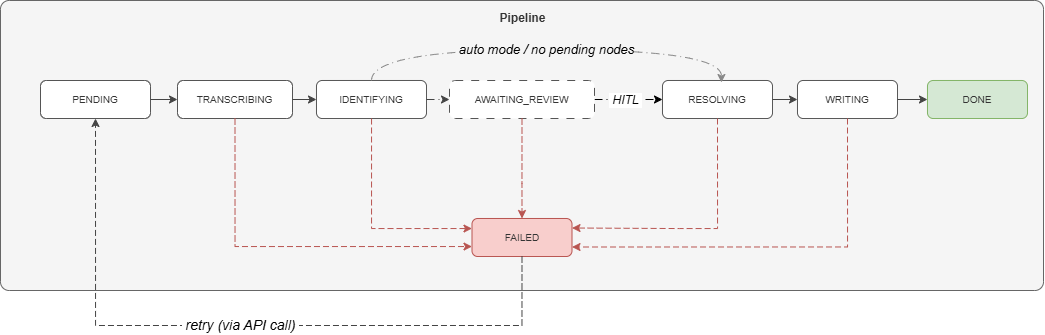
\includegraphics[width=\textwidth]{job_lifecycle.drawio.png}
  \caption{Ciclo de vida de un \textit{pipeline} en \textbf{Seshat}. \texttt{IDENTIFYING} y
           \texttt{RESOLVING} corresponden a las dos pasadas de extracción; el paso
           \textit{HITL} indica la revisión humana opcional; y en \texttt{WRITING} se
           persisten los nodos y sus relaciones en la base de conocimiento.
           \linebreak
           Las flechas discontinuas rojas señalan transiciones a error y la flecha inferior
           muestra el reintento mediante llamada a la \ac{API}.}
  \label{fig:job-lifecycle}
\end{figure}

\chapter{Implementación}
\label{ch:implementacion}

\section{Estructura del código y componentes}

El paquete \texttt{seshat} se organiza en cinco módulos (figura~\ref{fig:package-tree}):
\texttt{core/} contiene los modelos, configuración y utilidades; \texttt{infra/} agrupa
los adaptadores de sistemas externos; \texttt{app/} es la capa de aplicación;
\texttt{eval/} contiene los arneses de evaluación, que no forman parte del sistema en
producción; y \texttt{cli/} expone la línea de comandos.

\newcommand{\dtc}[1]{\hfill\makebox[10cm][l]{\textcolor{gray}{\texttt{\small\# #1}}}}

\begin{figure}[H]
\dirtree{%
  .1 seshat/.
  .2 app/.
  .3 agents/.
  .4 identification/.
  .4 resolution/.
  .3 pipeline/.
  .4 extraction/ \dtc{dos pasadas: identificación → RAG + resolución}.
  .4 ingestion/ \dtc{validación de audio/texto y normalización}.
  .3 platform/.
  .4 api/ \dtc{routers, autenticación, arranque}.
  .4 observability/ \dtc{trazas MLflow, latencia, presupuesto de tokens}.
  .4 worker/ \dtc{cola de tareas asíncrona en proceso}.
  .3 repositories/ \dtc{capa de acceso a datos que el pipeline consume}.
  .3 services/ \dtc{lógica de dominio: admin, graph, health, job}.
  .3 transcription/.
  .2 cli/.
  .2 core/.
  .3 config/.
  .3 models/ \dtc{nodos, relaciones, enumeraciones, modelos API}.
  .3 utils/ \dtc{retry, tokens, audio, logging}.
  .2 eval/ \dtc{tooling de calidad}.
  .3 calibration/ \dtc{meta-scorers para umbrales de confianza y retrieval}.
  .3 grounding/ \dtc{arnés del agente de verificación}.
  .3 grouping/ \dtc{arnés del agente de agrupación de decisiones}.
  .3 identification/ \dtc{arnés de extracción de nodos}.
  .3 resolution/ \dtc{arnés de resolución de relaciones}.
  .3 retrieval/ \dtc{arnés del motor de búsqueda}.
  .2 infra/.
  .3 blob\_store/.
  .3 knowledge\_store/ \dtc{nodos y relaciones}.
  .3 ops\_store/ \dtc{estado de trabajos y claves de API}.
  .3 secrets/ \dtc{resolución de credenciales}.
  .3 vector\_store/.
}
\caption{Estructura de paquetes de \textbf{Seshat}.}
\label{fig:package-tree}
\end{figure}

% ---------------------------------------------------------------------------
\section{Configuración centralizada}

Toda la configuración se centraliza en un único objeto \texttt{SeshatConfig}\footnote{La
referencia completa de parámetros y variables de entorno está disponible en
\url{https://github.com/josepmafe/seshat/blob/main/docs/configuration.md}.},
que hereda de \texttt{pydantic\_settings.BaseSettings}, con \texttt{\_\_} como separador de
anidamiento. Sus objetos anidados son subclases de \texttt{pydantic.BaseModel} planos de
modo que la resolución de variables de entorno ocurre exclusivamente en la raíz. El objeto
resultante es un \textit{singleton} inmutable cargado en el arranque del proceso.

Para los trabajos que requieren parámetros diferentes a los globales —por ejemplo, un umbral
de confianza más estricto o un modo automático activado—, la función \texttt{get\_request\_settings}
aplica una fusión profunda de un objeto \texttt{SeshatConfigOverride} opcional sobre el
\textit{singleton} base y devuelve un nuevo \texttt{SeshatConfig}. La fusión es recursiva a
cualquier profundidad: un campo no presente en el \textit{override} conserva su valor base en
todos los niveles. La configuración resultante —global o por trabajo— gobierna el comportamiento
de todas las etapas que se describen a continuación.

% ---------------------------------------------------------------------------
\section{Ingesta}
La ingesta comprende tres pasos: la validación del archivo de entrada, la transcripción de los
archivos de audio y la normalización de ambas rutas de entrada en un \texttt{TranscriptDocument}
común.

\subsection{Validación}
\label{sec:validacion-ingesta}

Los archivos de audio (.mp3, .wav, .m4a) pasan tres controles secuenciales antes de subirse a
blob storage:

\begin{enumerate}
  \item \textbf{Tamaño}: el archivo se rechaza si supera \texttt{max\_file\_bytes} (500~MiB por
        defecto).
  \item \textbf{Duración}: se extrae con \texttt{mutagen} y se rechaza si supera
        \texttt{max\_audio\_seconds} (dos horas por defecto).
  \item \textbf{Firma de bytes}: los primeros 12~bytes determinan el formato real
        (\textit{magic bytes}), que se contrasta con la extensión declarada; cualquier
        discrepancia se rechaza. La extensión por sí sola no es fiable al controlarla el cliente.
\end{enumerate}

El texto preformateado (.yaml, .yml, .json) solo requiere una comprobación de esquema y de
coherencia de la fecha de reunión, tras la cual el campo \texttt{content} se extrae directamente
como transcripción.

\subsection{Transcripción}

La transcripción de audio se delega en \texttt{AbstractTranscriber} —AssemblyAI por defecto—,
envuelta en \texttt{TrackingTranscriber} para acumular los segundos consumidos contra el
presupuesto de uso. El archivo original y la transcripción se persisten en blob storage como
artefactos de auditoría independientes de la base de conocimiento; si el trabajo falla más
adelante, ambos están disponibles para reintentar sin re-transcribir.

% ---------------------------------------------------------------------------
\section{Extracción multi-agente en dos pasadas}

La extracción es la fase de mayor coste computacional y el núcleo del sistema. Se articula en
dos pasadas secuenciales con un contrato estricto: todos los agentes de la primera pasada deben
completarse antes de que comience la segunda. Entre ambas se interpone la revisión humana opcional
(HITL): la primera pasada identifica y puntúa los nodos, y sólo para los nodos aprobados
—automática o manualmente— la segunda infiere las relaciones.

Todos los agentes comparten una base común que encapsula la invocación estructurada del LLM con
reintentos, y se descubren en tiempo de ejecución a partir de la configuración; habilitar o
deshabilitar un tipo de concepto es así un cambio de configuración y no de código. Sus prompts
de sistema, estáticos por tipo, se marcan además como cacheables a nivel de proveedor para
reducir coste y latencia. La arquitectura de clases de los agentes y el mecanismo de caché se
detallan en el anexo~\ref{anx:tecnico}.

Las cuatro subsecciones siguientes describen respectivamente la primera pasada —identificación y puntuación de
confianza—, y la segunda —recuperación y resolución—.

\subsection{Identificación}
\label{sec:agentes-identificacion}

La transcripción completa se envía en paralelo a cuatro agentes de identificación, uno por tipo
de concepto (figura~\ref{fig:identification-flow}). El \ac{MVP} no realiza segmentación previa: la
ventana de contexto de los modelos actuales es suficiente para transcripciones de reuniones
típicas. Cada agente recibe además un \textit{hint} ligero con los nodos de su mismo tipo ya
presentes en la base de conocimiento —título y resumen de los más recientes, acotado en
tokens—, lo que le permite ver ejemplos de nodos ya aprobados.

\begin{figure}[H]
  \centering
  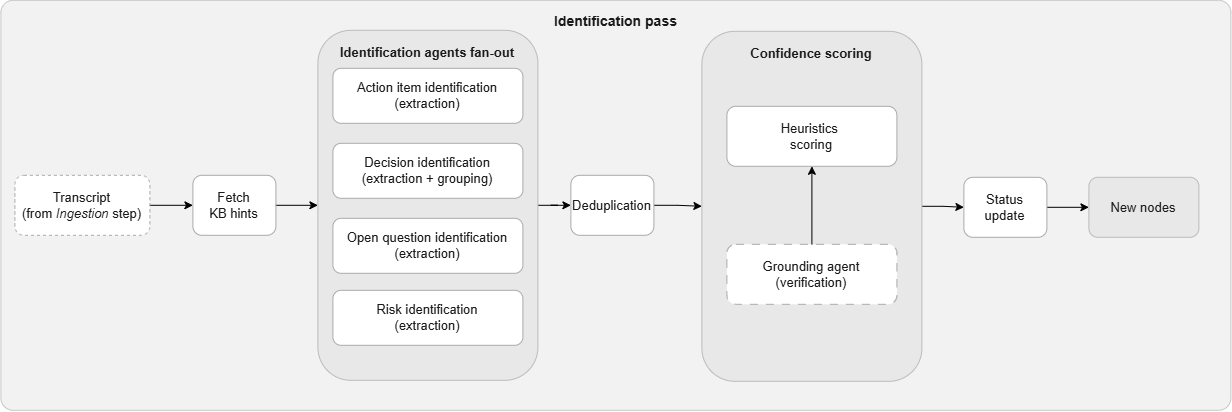
\includegraphics[width=\textwidth]{identification_flow.drawio.png}
  \caption{Flujo de la primera pasada de extracción. La transcripción normalizada en la ingesta
           alimenta el \textit{fan-out} de agentes de identificación —el de decisiones incluye
           además el paso de agrupación—; sus salidas se deduplican, se puntúan por confianza
           —heurísticas y, opcionalmente, verificación por \textit{grounding}— y reciben un estado
           de aprobación (pasos descritos en la sección~\ref{sec:confidence-scoring}) antes de
           persistirse como nodos nuevos.}
  \label{fig:identification-flow}
\end{figure}

Cada agente devuelve una lista de nodos estructurados mediante salida forzada con esquemas
Pydantic. Cada nodo queda anclado a una cita literal del texto fuente que lo respalda, lo que
reduce la alucinación y hace auditable cada afirmación. El diseño de los prompts de
identificación combina varias técnicas complementarias que se detallan en el anexo~\ref{anx:tecnico}.

Para el tipo \texttt{decision} se introduce un paso adicional de agrupación: la lista plana de
conceptos se organiza en grupos temáticos, de modo que el \textit{pipeline} genere un único
nodo por decisión consolidada en lugar de múltiples nodos fragmentados. El paso es configurable
por tipo, pues sólo las decisiones —que tienden a dispersarse a lo largo de un intercambio— se
benefician de forma clara; ante un fallo del agrupador, cada concepto retrocede a un grupo
unitario y ningún nodo se pierde.

Tras la ejecución de los agentes, los nodos con título idéntico y mismo tipo se fusionan
(\textit{deduplicación within-meeting}): el nodo más reciente en la salida del agente —que se
asume representa el estado final de la deliberación— absorbe los anteriores.

Opcionalmente, cada agente de identificación puede envolverse en una segunda pasada de
auto-revisión que valida y filtra sus propias salidas antes de puntuarlas; el mecanismo se
describe en el anexo~\ref{anx:tecnico}.

\subsection{Puntuación de confianza y estado de aprobación}
\label{sec:confidence-scoring}

Cada nodo recibe, antes de pasar a revisión, una puntuación de confianza en $[0,1]$: una señal
continua, resultado de la media ponderada de tres métricas heurísticas. Cada métrica aplica
reglas léxico-sintácticas sobre el análisis morfológico, de dependencias y de entidades que
produce el modelo \texttt{en\_core\_web\_sm} de \texttt{spaCy}:

\begin{equation}
  \text{confianza} = 0{,}3 \cdot s_{\text{cita}} + 0{,}3 \cdot s_{\text{título}} + 0{,}4 \cdot s_{\text{descripción}}
\end{equation}

donde $s_{\text{cita}}$ es una señal que satura a las 35 palabras de cita fuente. $s_{\text{título}}$ mide
la especificidad del título combinando tres señales —presencia de entidades nombradas, calificadores y
longitud, en ese orden de peso— que reflejan la importancia relativa de estas señales para distinguir
enunciados específicos de generales~\cite{louis2011specificity}. $s_{\text{descripción}}$ penaliza
multiplicativamente el lenguaje de cobertura, la voz pasiva y el tiempo futuro; los dos primeros son
marcadores léxicos de incertidumbre ya empleados en la detección de \textit{hedging}~\cite{farkas2010conll}.

Opcionalmente, el \texttt{GroundingAgent} actúa como compuerta binaria independiente: un modelo
ligero de un proveedor distinto al de los agentes de identificación —la configuración lo exige
para evitar errores correlacionados— juzga si la descripción está respaldada por la cita fuente.
Un nodo que falla la verificación es rechazado o marcado como pendiente de revisión,
independientemente de su puntuación heurística.

La política de aprobación automática combina ambas señales: si la puntuación supera el umbral
configurado y la verificación pasa (o está desactivada), el nodo se aprueba automáticamente con
\texttt{approval\_method=THRESHOLD}; en caso contrario el nodo queda en estado \texttt{AWAITING\_REVIEW}.
Con \texttt{auto\_mode=True}, todos los nodos cuya puntuación supere el umbral establecido se
aprueban sin revisión humana; los que no son rechazados automaticamente.

\subsection{Recuperación aumentada}
\label{sec:rag-resolucion}

El módulo de recuperación (RAG) opera en la segunda pasada, una vez que los nodos de la primera
han sido consolidados y aprobados. A diferencia del uso habitual de RAG, orientado a
responder preguntas fundamentando la respuesta en los documentos previamente ingeridos, aquí la
recuperación localiza los nodos preexistentes de la base de conocimiento con los que cada nodo
nuevo podría relacionarse.

Para cada nodo nuevo, el \texttt{NodeRetriever} construye una consulta a partir de su título y
descripción, la envía al \texttt{SearchEngine} con el umbral de similitud configurado y expande
los resultados con los vecinos directos del grafo (profundidad~1); por último, un reranking
opcional reordena los candidatos por relevancia. Un presupuesto de contexto
acotado en tokens limita el número total de candidatos para no sobrepasar la ventana del modelo
de resolución. La figura~\ref{fig:retrieval-flow} resume el recorrido de un nodo fuente a través
del recuperador.

\begin{figure}[H]
  \centering
  \includegraphics[width=\textwidth]{retrieval_flow.drawio.png}
  \caption{Flujo de recuperación para un nodo fuente, en su configuración completa (modo
           \texttt{HYBRID}). El \texttt{SearchEngine} combina una pata semántica (búsqueda densa,
           con expansión \textit{multi-query} opcional) y una pata dispersa por palabras clave,
           fundidas mediante RRF. El \texttt{NodeRetriever} obtiene los nodos de la base de
           conocimiento, los expande con sus vecinos directos y opcionalmente aplica un reranking
           (recuadro discontinuo) antes de devolver los nodos objetivo.}
  \label{fig:retrieval-flow}
\end{figure}

Un nodo puede recuperarse por dos vías complementarias, cada una con sus propias limitaciones. La
búsqueda \textbf{densa} (\textit{dense}) compara la consulta con los nodos en el espacio de
\textit{embeddings} y recupera por proximidad semántica: reconoce paráfrasis y sinónimos aunque
no compartan vocabulario, pero tiende a difuminar los términos raros y específicos. La búsqueda
\textbf{dispersa} (\textit{sparse}) casa términos literales y sobresale justo donde la densa se
diluye —nombres propios, herramientas o identificadores técnicos que el \textit{embedding}
promedia—, aunque no capta reformulaciones. \texttt{SearchEngine} expone ambas, y su combinación,
en tres modos de búsqueda configurables:

\begin{itemize}
  \item \texttt{SEMANTIC}: búsqueda densa por similitud coseno sobre pgvector. Es el modo por
        defecto. Opcionalmente admite un \textit{fan-out} multi-consulta: un LLM genera variantes
        de la consulta original —más abstractas, más específicas o con distinto vocabulario— y sus
        resultados se funden con \ac{RRF}~\cite{cormack2009rrf}, ampliando la cobertura frente a una
        única formulación.
  \item \texttt{KEYWORD}: búsqueda dispersa. Un LLM ligero destila primero la consulta a 3--6
        palabras clave discriminantes y la búsqueda se realiza sobre ellas; sin este paso, la
        coincidencia literal —que exige la presencia conjunta de todos los términos— se ahogaría
        en el vocabulario genérico de una consulta larga y devolvería poco o nada.
  \item \texttt{HYBRID}: combina la pata densa —con su \textit{fan-out} multi-consulta si está
        activo— y la dispersa, fusionándolas mediante \ac{RRF}, que las agrega por la posición
        de cada nodo en cada lista y no por su puntuación. Esto es deliberado: las similitudes
        coseno y las de texto viven en escalas distintas y no son directamente comparables,
        mientras que el rango sí lo es.
\end{itemize}

Sobre la lista devuelta por cualquiera de los modos puede aplicarse un \textit{reranking}
opcional. Mientras que la búsqueda densa aproxima la relevancia por la distancia entre vectores
calculados de forma independiente para consulta y candidato, un modelo \textit{cross-encoder}
procesa ambos textos de forma conjunta y estima su relevancia directamente, lo que reordena los
candidatos con mayor precisión a costa de una llamada adicional a un proveedor externo.

Por último, la recuperación es intencionalmente \textbf{multi-tipo}: un nodo de tipo
\texttt{decision} puede necesitar resolver relaciones frente a nodos de tipo \texttt{risk} o
\texttt{open\_question}, de modo que restringir la búsqueda al mismo tipo privaría de candidatos
válidos a los agentes de resolución cruzada.

\subsection{Agentes de resolución}
\label{sec:agentes-resolucion}

La resolución de relaciones opera en dos familias paralelas: \textbf{mismo tipo} y
\textbf{tipo cruzado} (figura~\ref{fig:resolution-flow}). En ambas, las relaciones son
\textbf{dirigidas} y se infieren en un único sentido: desde cada nodo nuevo (fuente) hacia los
nodos preexistentes de la base de conocimiento (destino) recuperados en la fase anterior. Los
nodos de reuniones previas no se reevalúan entre sí; sólo la llegada de un nodo nuevo dispara la
inferencia de relaciones, lo que mantiene el coste acotado al conocimiento incremental de cada
trabajo.

%\vspace{1.5cm}

\begin{figure}[H]
  \centering
  \includegraphics[width=\textwidth]{resolution_flow.drawio.png}
  \caption{Flujo de la segunda pasada. Para cada nodo fuente de la primera pasada se recuperan
           sus nodos objetivo (recuperación descrita en la sección~\ref{sec:rag-resolucion}); el
           par fuente–objetivos se envía en paralelo a las familias de resolución de mismo tipo
           (un agente por tipo) y de tipo cruzado (hasta nueve pares activos). Un paso de
           validación mediante reglas heurísticas filtra las relaciones inferidas antes de
           persistirlas.}
  \label{fig:resolution-flow}
\end{figure}

Los agentes de mismo tipo clasifican cada nodo nuevo frente a los candidatos recuperados de la
base de conocimiento en una de las relaciones aplicables a su tipo o sin relación. Por ejemplo,
para un nodo de tipo \texttt{decision}, las relaciones permitidas del mismo tipo son
\texttt{supersedes}, \texttt{amends} y \texttt{conflicts\_with} (el conjunto completo por tipo se
recoge en la tabla~\ref{tab:rel-matrix} del anexo~\ref{anx:tecnico}). Además, el prompt establece
criterios operativos precisos: \texttt{supersedes} requiere que la decisión previa quede
funcionalmente obsoleta; \texttt{amends} implica que la decisión previa permanece vigente pero es
matizada o restringida; \texttt{conflicts\_with} requiere que ambas decisiones sean activas
simultáneamente e incompatibles. Ante ambigüedad entre \texttt{amends} y \texttt{supersedes}, el
sistema prefiere \texttt{amends} como clasificación menos destructiva.

Los agentes de tipo cruzado detectan relaciones entre nodos de tipos distintos:
\texttt{mitigates}, \texttt{blocks} y \texttt{resolves}. Por ejemplo, una \texttt{decision} puede
mitigar (\texttt{mitigates}) un \texttt{risk} o resolver (\texttt{resolves}) una
\texttt{open\_question}. El esquema de relaciones restringe qué pares de tipos pueden evaluarse:
de los 12 pares dirigidos posibles entre tipos distintos, el \ac{MVP} habilita los 9 cuyas fronteras
semánticas son más nítidas, materializados como instancias de agente fijas; los restantes quedan
fuera de alcance por ser más ambiguos de clasificar de forma fiable. La tabla~\ref{tab:rel-matrix}
del anexo~\ref{anx:tecnico} detalla los pares habilitados.

Cuando un agente tiene incertidumbre genuina entre dos relaciones, puede señalarlo mediante el
campo opcional \texttt{alt\_rel\_type}. Este campo es la interfaz entre el agente de resolución
y una segunda pasada de auto-revisión opcional que arbitra los casos ambiguos, análoga a la de
identificación y detallada igualmente en el anexo~\ref{anx:tecnico}.

Tras ambas llamadas paralelas, un paso de validación heurística descarta las relaciones
malformadas —dirección incorrecta, incompatibilidades de tipo, violaciones del esquema— y las
registra sin interrumpir el trabajo.

% ---------------------------------------------------------------------------
\section{Orquestación y ciclo de vida del pipeline}
\label{sec:orquestacion}

Las dos pasadas de extracción descritas hasta aquí no se invocan directamente: son etapas de un
\textit{pipeline} que la \ac{API} encola y un \textit{worker} asíncrono ejecuta. Cada \textit{pipeline}
avanza por la máquina de estados descrita en la figura~\ref{fig:job-lifecycle}, desde su recepción
hasta la persistencia de los resultados.

\subsection{API y creación del pipeline}

La \ac{API} REST (FastAPI) es el único punto de entrada programático al sistema. Un \textit{pipeline}
se crea enviando un archivo de entrada, que la \ac{API} valida y persiste junto con el registro del
trabajo antes de encolarlo para su procesamiento asíncrono: la petición retorna de inmediato, sin
esperar al resultado. El resto de operaciones del ciclo de vida —consultar estado, recuperar
resultados, aprobar la revisión o reintentar un \textit{pipeline} fallido— se exponen como
\textit{endpoints} sobre el mismo recurso; la referencia completa de la \ac{API} se recoge en el
anexo~\ref{anx:api-reference}. El \texttt{JobService} concentra esta lógica de dominio y se apoya
en repositorios que encapsulan el acceso a datos, de modo que ningún \textit{endpoint} consulta la
base de datos directamente.

En la creación se aplican además dos salvaguardas: un control de duplicados por
\textit{hash} del contenido —que evita re-procesar un archivo ya ingerido salvo forzado
explícito— y límites de tasa por usuario y de concurrencia global, que protegen el presupuesto
de tokens frente a envíos masivos.

\subsection{Worker asíncrono y máquina de estados}

El \textit{worker} consume los \textit{pipelines} encolados y los conduce a través de los estados
del ciclo de vida, actualizando el estado persistido en cada transición para que la \ac{API} pueda
reportarlo. La ejecución se divide en dos tramos separados por la revisión humana. El primero
—ingesta, transcripción e identificación— termina dejando el \textit{pipeline} en
\texttt{AWAITING\_REVIEW}. El segundo —recuperación, resolución y escritura— sólo arranca una vez
aprobados los nodos. Cuando el modo automático está activo, o cuando ningún nodo queda pendiente
de revisión, el segundo tramo se encadena sin intervención manual.

El \textit{worker} está diseñado para tolerar fallos sin dejar la base de conocimiento en un
estado inconsistente. La escritura final de nodos y relaciones es una única transacción, de modo
que un fallo en cualquier punto no deja estado parcial. Además, cuando un \textit{pipeline} falla
queda en estado \texttt{FAILED} conservando su archivo original; la operación de reintento lo
recupera del almacenamiento y vuelve a ejecutar el \textit{pipeline} completo desde la transcripción,
sin reutilizar el trabajo ya realizado —una reanudación consciente del progreso queda como trabajo
futuro (sección~\ref{sec:trabajo-futuro})—. Por último, los \textit{pipelines} interrumpidos por una
caída del proceso durante la escritura se detectan y marcan como recuperables en el siguiente arranque.

\subsection{Revisión humana (HITL)}

En \texttt{AWAITING\_REVIEW}, el \textit{pipeline} se detiene a la espera de que un revisor decida
el destino de los nodos extraídos. Las decisiones se envían en una única petición al
\textit{endpoint} de aprobación, que admite dos mecanismos combinables. El primero es una
aprobación masiva por umbral: aprueba de una vez todos los nodos pendientes cuya confianza supere
un valor dado. El segundo son decisiones individuales: aprobar, rechazar o editar un nodo concreto.
Cuando se usan juntos, la regla masiva se aplica primero y las decisiones individuales se superponen
a su resultado, de modo que el revisor puede, por ejemplo, aprobar en bloque todo lo que supere el
umbral y luego rechazar o corregir los casos puntuales que lo requieran. Las ediciones y aprobaciones
registran quién y cuándo, distinción que sostiene la trazabilidad descrita a continuación. Una vez
enviadas las decisiones, el \textit{pipeline} transita a la fase de resolución y el \textit{worker}
retoma el segundo tramo.

% ---------------------------------------------------------------------------
\section{Mecanismos de seguridad}

\subsection{Control de acceso y autenticación}

Todos los \textit{endpoints} de la \ac{API} requieren una clave de \ac{API} en la cabecera
\texttt{X-API-Key}. Las claves se almacenan como hashes bcrypt (factor de coste~12); el texto
plano nunca se persiste. La validación de cada petición usa comparación en tiempo constante para
prevenir ataques de temporización.

El modelo de roles es jerárquico; cada nivel hereda los permisos del anterior:

\begin{equation*}
  \texttt{viewer} \;\subset\; \texttt{reviewer} \;\subset\; \texttt{operator} \;\subset\; \texttt{admin}
\end{equation*}

\texttt{viewer} sólo consulta la base de conocimiento; \texttt{reviewer} es el nivel mínimo para
enviar un \textit{pipeline} y para decidir sobre los nodos en revisión —aprobarlos, rechazarlos o
editarlos—. Activar el modo automático se sitúa también en este nivel, pues equivale a aprobar en
bloque sin revisión manual. Las acciones más sensibles se reservan a niveles superiores: los
\textit{overrides} de configuración por trabajo requieren \texttt{operator}, mientras que las
operaciones de borrado y la re-ingesta forzosa —que elimina nodos existentes— requieren
\texttt{admin}. La provisión de claves de \ac{API} queda al margen de esta jerarquía: se realiza a
través de un router \texttt{/admin} separado, autenticado con una clave raíz (\textit{root})
almacenada en Secrets Manager en lugar de con una clave de usuario.

\subsection{Validación de entradas}

Más allá del control de acceso, el sistema trata como hostiles sus dos entradas no controladas. El
archivo del cliente se valida en la frontera de la \ac{API} por firma de bytes
(sección~\ref{sec:validacion-ingesta}) en fallo cerrado: una entrada inválida se rechaza antes de
crear el \textit{pipeline} y no deja ni trabajo encolado ni artefacto almacenado. El texto de la
transcripción, que llega a los agentes, se aísla frente a la inyección de prompts mediante los
delimitadores XML del anexo~\ref{anx:tecnico}, reforzados por la salida estructurada forzada:
aunque el modelo procese contenido malicioso, el resultado debe ajustarse al esquema Pydantic para
no ser descartado.

% ---------------------------------------------------------------------------
\section{Observabilidad y trazabilidad}
\label{sec:observabilidad}

La observabilidad es una preocupación transversal en un sistema construido sobre \ac{LLM}: las
llamadas a los modelos son costosas, no deterministas y ocurren en paralelo, por lo que sin
instrumentación es difícil diagnosticar un fallo, atribuir un coste o justificar una afirmación
extraída. \textbf{Seshat} aborda esto en tres planos: el trazado de la ejecución, la medición del
consumo con enforcement de presupuesto, y la trazabilidad del conocimiento producido.

\subsection{Trazado de la ejecución}

MLflow~3 actúa como \textit{backbone} de observabilidad. La instrumentación de las llamadas a los
agentes es automática: \texttt{mlflow.langchain.autolog()} captura prompts, respuestas, uso de
tokens y latencia sin código adicional en los agentes, emitiendo cada llamada como un \textit{span}
de \ac{OTel}, el estándar abierto de trazado distribuido. Cada \textit{pipeline} abre un
\textit{run} de MLflow al arrancar; su identificador se
expone en la consulta de estado del trabajo, de modo que el operador puede saltar directamente a la
traza completa de la ejecución.

\subsection{Medición del consumo y presupuesto}

Sobre el trazado automático, \textbf{Seshat} añade una capa propia de medición que acumula, por
etapa del \textit{pipeline}, los tokens de entrada, salida y caché del LLM, los tokens de
\textit{embeddings} y de \textit{reranking}, y los segundos de audio transcritos, junto con
percentiles de latencia por llamada (media, p95 y máximo). Estas métricas se registran en MLflow y
hacen comparables el coste y el rendimiento entre versiones del sistema.

Esta capa no es meramente informativa: aplica un presupuesto de consumo. Cada etapa acumula su uso
contra unos límites configurables y aborta la ejecución si los rebasa, lo que acota el gasto ante
transcripciones anómalas o bucles inesperados. El control de gasto real recae así sobre estos
límites de tokens, y no sobre tablas de precios que requerirían mantenimiento; los costes
monetarios se estiman de forma informativa en la interfaz de MLflow. Los detalles de
implementación de esta capa —su propagación transparente a los agentes concurrentes y los
envoltorios de medición— se describen en el anexo~\ref{anx:observabilidad}.

\subsection{Trazabilidad del conocimiento}

Al margen de la instrumentación de ejecución, cada nodo conserva la traza de su origen y de su
manipulación posterior. La cita literal del texto fuente (\texttt{quote\_anchors}) que originó el
nodo hace auditable cualquier afirmación extraída. Las correcciones humanas en revisión quedan
registradas en los campos \texttt{corrected\_by} y \texttt{corrected\_at}, distinguiendo el
contenido corregido del generado automáticamente, y las anulaciones (\textit{overrides}) de
operadores y administradores exigen justificación escrita, almacenada en
\texttt{correction\_reason}.

% ---------------------------------------------------------------------------
\section{Despliegue e infraestructura}

\subsection{Contenedores Docker}

El sistema se orquesta con Docker Compose en seis servicios: \texttt{postgres}
(PostgreSQL~17 con pgvector), \texttt{mlflow} (observabilidad, con \textit{backend} SQLite),
\texttt{localstack} (emulación de S3 y Secrets Manager), \texttt{migrate} (aplica las migraciones
de esquema mediante Alembic y termina), \texttt{seshat-api} (la \ac{API} FastAPI, que aloja además el \textit{worker}
asíncrono en proceso) y \texttt{seshat-ui} (la interfaz de revisión en Streamlit). El arranque
está ordenado por comprobaciones de salud: la \ac{API} sólo se inicia cuando Postgres, LocalStack y
MLflow están operativos y las migraciones han concluido.

La \ac{API} y las migraciones se construyen desde un mismo \textit{Dockerfile} multietapa —comparten la
capa de dependencias y difieren sólo en la etapa final—, de modo que ambas ejecutan exactamente el
mismo entorno. La configuración se inyecta por variables de entorno mediante el separador de
anidamiento de pydantic-settings; los secretos —incluida la cadena de conexión de Postgres, bajo
la clave \texttt{seshat/postgres\_url}— se resuelven en el arranque desde Secrets Manager, de modo
que el mismo código se ejecuta en desarrollo (LocalStack) y en producción (AWS real) sin ramas
condicionales.

\subsection{Integración continua}
\label{sec:ci}

Cada \textit{push} a la rama principal y cada \textit{pull request} dispara una canalización de
\ac{CI} (GitHub Actions) que actúa como guardián de calidad antes de la fusión. La canalización
arranca con una etapa de \textit{linting} —formato y reglas estáticas con \textit{ruff}, más
comprobación de tipos con \textit{mypy}— de la que dependen las demás: si el estilo o los tipos
fallan, no se malgasta cómputo en las pruebas. Superada esa puerta, las pruebas unitarias y las de
integración (sección~\ref{sec:tests}) se ejecutan en paralelo; estas últimas levantan los mismos
contenedores de Docker Compose de la sección anterior, de modo que se validan contra Postgres, LocalStack y
MLflow reales, y exigen una cobertura de ramas mínima del 80\,\%. Una última etapa, sólo en las \textit{pull requests}, publica
como comentario métricas de complejidad ciclomática y de mantenibilidad del código, dando
visibilidad a la deuda técnica en el momento de la revisión.

La canalización ejecuta deliberadamente todas las pruebas salvo las marcadas como dependientes de
un \ac{LLM} en vivo: reproducir la aleatoriedad y el coste de las llamadas reales al modelo en cada
\textit{commit} no es ni fiable ni económico. La evaluación de la calidad de los agentes recae por
ello en el \textit{gate} descrito en el capítulo~\ref{ch:evaluacion}, que se ejecuta de forma
deliberada fuera de la \ac{CI} y cuyo veredicto la \ac{API} comprueba en el arranque.

\chapter{Evaluación del Sistema}
\label{ch:evaluacion}

\section{Estrategia de evaluación}

Evaluar un sistema construido sobre \ac{LLM} plantea una dificultad propia: sus componentes no
son deterministas —una misma entrada puede producir salidas distintas entre ejecuciones— y sus
fallos son silenciosos, pues una alucinación tiene la misma forma que una extracción correcta.
Sin una medición sistemática y repetible es imposible saber si un cambio de \textit{prompt}, de
modelo o de umbral mejora el sistema o lo degrada. La estrategia de evaluación de \textbf{Seshat}
responde a esa dificultad con dos decisiones: medir por separado cada etapa no determinista, y
convertir el resultado de esa medición en una condición de despliegue.

La calidad se mide con cinco arneses independientes, uno por cada etapa del \textit{pipeline} con
comportamiento no determinista: identificación, agrupación, \textit{grounding}, recuperación
(\textit{retrieval}) y resolución de relaciones. La elección de esas cinco etapas no es arbitraria:
el resto del \textit{pipeline}  es determinista y queda cubierto por las pruebas unitarias y de
integración habituales, donde una salida incorrecta delata un error de código. Sólo estas cinco
etapas, cuya salida depende de un \ac{LLM} o de la similitud vectorial, pueden degradarse en
silencio ante un cambio de \textit{prompt}, de modelo o de corpus, sin que ninguna prueba
convencional lo advierta; por eso son las que exigen medirse contra una referencia.

Cada arnés ejecuta el componente real del sistema contra un corpus de casos con verdad de referencia,
y produce métricas de precisión y \textit{recall} adaptadas a la tarea que evalúa, calculadas por
\textit{scorers} deterministas propios y no por un LLM como juez, para que el veredicto sea
reproducible. Lo que se mide es así exactamente lo que se ejecuta en producción. Aislar cada etapa
cumple además un segundo
propósito, más allá de la cobertura: atribuir una regresión a su origen. Como la resolución opera
sobre los candidatos que le entrega la recuperación, un fallo observado de principio a fin podría
nacer en cualquiera de las dos; medirlas por separado, cada una contra su propia verdad de referencia,
distingue si el problema está en \emph{qué} se recuperó o en \emph{cómo} se clasificó.

Los cinco arneses vuelcan su veredicto —una métrica por criterio, con su marca de aprobado o
suspenso— a un fichero de \textit{gate} común que agrega los resultados de todos los arneses
ejecutados. Ese fichero no es un mero informe: la \ac{API} se niega a arrancar si el \textit{gate}
no está presente o no ha pasado, de manera que el sistema no puede procesar datos reales con
una calidad por debajo de los objetivos fijados. Los umbrales que definen ese aprobado residen
en código, no en configuración, para que modificarlos exija un cambio revisable y no un simple
ajuste de entorno.

La tabla~\ref{tab:eval-gate-criteria} recoge el contrato completo de calidad: qué mide cada arnés,
qué umbral debe superar cada métrica para aprobar y si su incumplimiento bloquea el arranque del
sistema. No todas las métricas medidas condicionan el \textit{gate}: algunas se registran en
MLflow solo con fines de observabilidad, pues resultan demasiado estrictas o poco discriminantes
para servir de criterio de bloqueo —una distinción que se justifica caso por caso en los
resultados de cada arnés.

\begin{table}[htbp]
  \centering
  \small
  \setlength{\tabcolsep}{12pt}
  \begin{tabular}{l l l l}
    \toprule
    \textbf{Arnés} & \textbf{Métrica} & \textbf{Umbral} & \textbf{Bloqueante} \\
    \midrule
    Identificación & precisión (por tipo)  & $\geq$0.75--0.85 & Sí \\
                   & recall (por tipo)     & $\geq$0.75--0.85 & Sí \\
                   & tasa espuria (por tipo) & $\leq$0.10--0.15 & Sí \\
                   & F1                    & ---              & No \\
    \addlinespace
    \cmidrule[0.02em]{1-4}
    Agrupación & \texttt{group\_hit\_rate} & $\geq$0.80 & Sí \\
               & \texttt{exact\_match}     & ---        & No \\
    \addlinespace
    \cmidrule[0.02em]{1-4}
    \textit{Grounding} & precisión & $\geq$0.85 & Sí \\
                       & recall    & $\geq$0.80 & Sí \\
    \addlinespace
    \cmidrule[0.02em]{1-4}
    Recuperación & \texttt{recall@5}    & $\geq$0.70 & Sí \\
                 & \texttt{mrr@5}       & $\geq$0.75 & Sí \\
                 & \texttt{precision@5} & ---        & No \\
    \addlinespace
    \cmidrule[0.02em]{1-4}
    Resolución & precisión (por tipo) & $\geq$0.80 & Sí \\
               & recall (por tipo)    & $\geq$0.80 & Sí \\
               & F1                   & ---        & No \\
    \bottomrule
  \end{tabular}
  \caption{Criterios del \textit{gate} de evaluación: métricas medidas por cada arnés, umbral de
           aprobado y si su incumplimiento impide el arranque del sistema. Los umbrales de
           identificación varían según el tipo de concepto; se indica su rango y los valores
           exactos por tipo se recogen en la tabla~\ref{tab:eval-identification}.}
  \label{tab:eval-gate-criteria}
\end{table}

La arquitectura interna de los arneses —el emparejador \textit{greedy} de identificación, el
mecanismo de caché compartido y el diseño de las trazas de MLflow— se detalla en el
anexo~\ref{anx:harnesses-eval}; este capítulo se centra en qué se mide, con qué corpus y con qué
resultado.

\section{Corpus sintético de evaluación}

En ausencia de transcripciones reales de reuniones —por razones de privacidad y disponibilidad—
el corpus de referencia se genera con apoyo de un LLM: cada fichero YAML describe un escenario
de reunión sintético junto con la salida esperada del componente bajo prueba. Un corpus
curado a partir de datos reales sería preferible, pero no es viable en esta fase del proyecto.
A pesar de ello, todos los casos se diseñan y revisan manualmente para compensar parcialmente
esta limitación.

Cada arnés organiza su corpus en \textit{tiers}: familias de casos que comparten un mismo
propósito de prueba y cuyo nombre de fichero lleva el \textit{tier} como prefijo explícito,
seguido de un número de secuencia y de una descripción breve del escenario. Así, un fichero
como \texttt{boundary\_001\_decision\_coexists\_with\_risk.yaml} revela sin abrirlo tanto su
rol como la ambigüedad que ejercita: una decisión y un riesgo que conviven en el mismo fragmento.
Esta convención permite auditar de un vistazo la cobertura del corpus y añadir casos nuevos
sin romper su organización. La tabla~\ref{tab:eval-corpus} resume la composición actual:

\begin{table}[htbp]
  \centering
  \small
  \begin{tabularx}{\textwidth}{l >{\raggedright\arraybackslash}X r}
    \toprule
    \textbf{Tier} & \textbf{Rol del caso} & \textbf{Casos} \\
    \midrule
    \multicolumn{2}{l}{\textbf{Identificación}} & \textbf{31} \\
    \cmidrule[0.02em]{1-3}
    \texttt{happy}       & Transcripciones claras y cooperativas; la extracción debe acertar con alta confianza & 10 \\
    \texttt{boundary}    & Interacciones entre tipos donde el agente tiende a alucinar o a suprimir de más & 8 \\
    \texttt{negative}    & Uno o más agentes deben devolver vacío; ejercita los criterios de rechazo & 7 \\
    \texttt{adversarial} & Trampas de inyección de \textit{prompt} y de atribución de responsable & 3 \\
    \texttt{realistic}   & Transcripciones largas y naturales, con deriva temática y varios locutores & 3 \\
    \addlinespace
    \multicolumn{2}{l}{\textbf{Resolución}} & \textbf{44} \\
    \cmidrule[0.02em]{1-3}
    \texttt{simple}    & Un nodo fuente y uno de la base: una única relación esperada evidente, o ninguna & 23 \\
    \texttt{null}      & Salida esperada sin relaciones; nodos temáticamente próximos pero no vinculados & 11 \\
    \texttt{multi}     & Un nodo fuente frente a varios candidatos; algunos relacionados, otros no & 7 \\
    \texttt{realistic} & Contexto completo de reunión: varios nodos fuente y de la base, mezcla de tipos & 3 \\
    \addlinespace
    \multicolumn{2}{l}{\textbf{Recuperación}} & \textbf{40} \\
    \cmidrule[0.02em]{1-3}
    \texttt{same\_type}  & \textit{Pool} de un solo tipo; consulta y candidato del mismo tipo & 4 \\
    \texttt{cross\_type} & \textit{Pool} de un solo tipo; consulta y candidato de tipos distintos & 9 \\
    \texttt{realistic}   & \textit{Pool} mixto de los cuatro tipos; distribución realista de producción & 17 \\
    \texttt{negative}    & \textit{Pool} mixto sin candidatos relevantes; nada debería situarse arriba & 10 \\
    \addlinespace
    \multicolumn{2}{l}{\textbf{Agrupación}} & \textbf{8} \\
    \cmidrule[0.02em]{1-3}
    \texttt{singleton} & Cada ítem debe formar su propio grupo; no hay fusión & 2 \\
    \texttt{merge}     & Varios ítems que deben fundirse en un único grupo & 2 \\
    \texttt{mixed}     & Combinación de ítems que se fusionan y de ítems que quedan sueltos & 2 \\
    \texttt{realistic} & Transcripciones largas; agrupación de extremo a extremo & 2 \\
    \addlinespace
    \multicolumn{2}{l}{\textbf{\textit{Grounding}}} & \textbf{12} \\
    \cmidrule[0.02em]{1-3}
    \texttt{faithful}      & La cita respalda genuinamente la afirmación; el agente no debe rechazar de más & 5 \\
    \texttt{hallucination} & La afirmación añade hechos ausentes en la cita; el agente debe detectar la fabricación & 6 \\
    \texttt{adversarial}   & Trampas de inyección de \textit{prompt} y de manipulación de identidad & 1 \\
    \bottomrule
  \end{tabularx}
  \caption{Composición del corpus de evaluación por arnés y \textit{tier}, con el rol que cumple
           cada \textit{tier} y su número de casos.}
  \label{tab:eval-corpus}
\end{table}

Los \textit{tiers} \texttt{negative} y \texttt{null} merecen una mención aparte: comprueban que
el sistema no extrae ni resuelve nada cuando no corresponde, un aspecto que la precisión sólo
capta indirectamente. Los \texttt{boundary} y \texttt{adversarial}, por su parte, documentan
dentro del propio fichero por qué un caso es ambiguo; esa nota sobrevive a los cambios de
\textit{prompt} y evita que una simple oscilación de puntuación se confunda con una regresión
real.

\section{Métricas y resultados por arnés}

Los resultados de esta sección corresponden a la última ejecución del \textit{gate} sobre el
corpus descrito (\texttt{eval\_gate.json}). Las tablas recogen los valores medidos; el umbral que
cada métrica debe superar y su carácter bloqueante figuran en el contrato de la
tabla~\ref{tab:eval-gate-criteria}. En identificación, cuyos umbrales varían por tipo de concepto,
se repiten junto a cada valor para facilitar la comparación directa.

Todos los arneses puntúan con \textit{scorers} deterministas propios, sin recurrir a un LLM como
juez: solapamiento difuso de citas y campos en identificación, comparación de conjuntos en
agrupación, matrices de confusión en \textit{grounding}, métricas de posición en \textit{retrieval}
y coincidencia exacta de ternas en resolución. La decisión es deliberada. Un juez basado en LLM
reintroduciría en la propia medición el no determinismo y potenciales alucinaciones, y volvería el
veredicto irreproducible; un \textit{scorer} determinista, en cambio, produce la misma puntuación
ante la misma predicción.

El no determinismo residual proviene entonces del \textit{pipeline} evaluado, no del instrumento de
medida: incluso a temperatura cero, la salida del \ac{LLM} puede variar entre ejecuciones por la
no asociatividad de la aritmética en coma flotante bajo ejecución en
paralelo~\cite{goldberg1991floating}. Que el instrumento sea determinista es condición necesaria
para que ese ruido no se confunda con el del sistema, para que el \textit{gate} sea un criterio
estable y para el requisito de evaluación funcionalmente determinista del
capítulo~\ref{ch:requisitos-diseno}.

\subsection{Identificación}

El arnés de identificación ejecuta la primera pasada de extracción sobre la transcripción de cada
caso y empareja los nodos extraídos con los esperados para contarlos como aciertos, falsos
positivos o falsos negativos; el emparejador que decide esas correspondencias se describe en el
anexo~\ref{anx:harnesses-eval}. De ese recuento salen la precisión y el \textit{recall} por tipo
de concepto. Junto a ellos se registra la \textbf{tasa espuria}, que mide un fallo distinto: la
extracción de un tipo de concepto que no debería aparecer en el caso. Se calcula sobre los casos
donde un tipo está ausente de la verdad de referencia, como la fracción de ellos en los que el
agente extrajo al menos un nodo de ese tipo; captura así la contaminación entre tipos que la
precisión, calculada por tipo, no refleja.

\begin{table}[H]
  \centering
  \begin{tabular}{lccc}
    \toprule
    \textbf{Tipo} & \textbf{Precisión} & \textbf{Recall} & \textbf{Tasa espuria} \\
    \midrule
    \texttt{decision}      & 0.964 ($\geq$0.80) & 0.893 ($\geq$0.80) & 0.000 ($\leq$0.10) \\
    \texttt{risk}          & 0.850 ($\geq$0.75) & 1.000 ($\geq$0.80) & 0.000 ($\leq$0.10) \\
    \texttt{action\_item}  & 0.895 ($\geq$0.85) & 0.947 ($\geq$0.85) & 0.077 ($\leq$0.10) \\
    \texttt{open\_question}& 0.867 ($\geq$0.75) & 0.867 ($\geq$0.75) & 0.111 ($\leq$0.15) \\
    \bottomrule
  \end{tabular}
  \caption{Precisión, recall y tasa espuria de identificación por tipo de concepto. Cada valor
           está promediado sobre los casos del corpus.}
  \label{tab:eval-identification}
\end{table}

Los cuatro tipos superan su umbral. El umbral de tasa espuria de \texttt{open\_question} es
deliberadamente más laxo (0.15 frente a 0.10): la frontera entre una pregunta abierta y un
riesgo o una decisión pendiente es genuinamente ambigua en el lenguaje conversacional, y así
queda reflejado también en su tasa espuria observada, la más alta de los cuatro tipos.

\subsection{Agrupación}

La agrupación es el paso que consolida las decisiones fragmentadas de la primera pasada en un
único nodo por decisión (sección~\ref{sec:agentes-identificacion}). El agente recibe la lista
plana de conceptos extraídos y la reparte en grupos, cada uno destinado a fundirse en un solo
nodo, de manera que su salida es una partición $P$ de esos conceptos que se contrasta con la
partición de referencia $E$. Ambas se tratan como conjuntos de grupos, y cada grupo como un
conjunto de conceptos, por lo que ni el orden de los grupos ni el de los conceptos dentro de
cada grupo influye en la puntuación. Sobre ellas se definen dos métricas, que comparan las
particiones a distinta resolución:

\begin{equation}
  \text{exact\_match} =
  \begin{cases}
    1 & \text{si } P = E, \\
    0 & \text{en caso contrario,}
  \end{cases}
  \qquad
  \text{group\_hit\_rate} = \frac{\lvert P \cap E \rvert}{\lvert E \rvert}.
\end{equation}

La primera es una medida de todo o nada: vale 1 sólo si la partición predicha coincide íntegramente
con la esperada y cae a 0 en cuanto un solo grupo difiere. La segunda concede crédito parcial: es la
fracción de grupos esperados que reaparecen exactamente en la predicción.

\begin{table}[H]
  \centering
  \begin{tabular}{lc}
    \toprule
    \textbf{Métrica} & \textbf{Valor} \\
    \midrule
    \texttt{exact\_match}    & 0.750 \\
    \texttt{group\_hit\_rate}& 0.850 \\
    \bottomrule
  \end{tabular}
  \caption{Resultados del arnés de agrupación. Cada valor está promediado sobre los casos del
           corpus.}
  \label{tab:eval-grouping}
\end{table}

Sólo \texttt{group\_hit\_rate} condiciona el \textit{gate}; \texttt{exact\_match} se registra pero
no bloquea, por ser demasiado estricta a medida que crece el número de grupos por caso: un único
grupo mal formado hunde toda la puntuación del ejemplo aunque el resto sea correcto. La brecha entre
ambos valores observados —0.750 frente a 0.850— es precisamente esa penalización: el agente acierta
la mayoría de los grupos, pero rara vez reproduce la partición entera sin un solo desajuste, y es
\texttt{group\_hit\_rate} quien recoge ese acierto parcial que \texttt{exact\_match} descarta.

\subsection{Grounding}

El \textit{grounding} es la compuerta opcional que, durante la puntuación de confianza, verifica
si la cita de un nodo respalda su título y descripción
(sección~\ref{sec:confidence-scoring}). Su arnés mide si el agente emite ese juicio correctamente:
cada nodo del corpus lleva anotado si su cita lo respalda o no, y la predicción del agente se
clasifica en la matriz de confusión (verdaderos y falsos positivos y negativos) que se agrega en
precisión y \textit{recall}.

\begin{table}[H]
  \centering
  \begin{tabular}{lc}
    \toprule
    \textbf{Métrica} & \textbf{Valor} \\
    \midrule
    Precisión & 1.000 \\
    Recall    & 1.000 \\
    \bottomrule
  \end{tabular}
  \caption{Resultados del arnés de \textit{grounding}. Ambos valores se agregan sobre todos los
           nodos del corpus en una única matriz de confusión.}
  \label{tab:eval-grounding}
\end{table}

El resultado perfecto debe leerse con cautela: el corpus de \textit{grounding} es de los más pequeños
de los cinco (12 casos), de modo que el 1.000 significa «sin fallos observados en 12 casos», no una
garantía de perfección; un único caso adicional podría desplazar la métrica de forma apreciable.

\subsection{Recuperación (retrieval)}

Los tres arneses anteriores cubren la primera pasada de extracción; los dos siguientes evalúan la
segunda, que arranca recuperando los nodos con los que cada nodo nuevo podría relacionarse
(sección~\ref{sec:rag-resolucion}). El arnés de recuperación siembra el almacén vectorial con los
candidatos de cada caso y comprueba si la búsqueda sitúa los nodos relevantes entre los cinco
primeros resultados.

Es también la etapa más configurable del \textit{pipeline}: el modo de búsqueda, los modelos de
lenguaje de sus patas densa y dispersa —con sus propios parámetros— y el modelo de
\textit{embeddings} son todos intercambiables (sección~\ref{sec:rag-resolucion}), y cada
combinación desplaza el equilibrio entre latencia, coste y calidad. Las cifras de esta sección no
son, por tanto, un techo del componente, sino el resultado de una configuración concreta, elegida
por ofrecer un buen compromiso entre velocidad y rendimiento.

\begin{table}[H]
  \centering
  \begin{tabular}{lc}
    \toprule
    \textbf{Métrica} & \textbf{Valor} \\
    \midrule
    \texttt{recall@5}    & 0.742 \\
    \texttt{precision@5} & 0.560 \\
    \texttt{mrr@5}       & 0.944 \\
    \bottomrule
  \end{tabular}
  \caption{Resultados del arnés de recuperación. Cada valor está promediado sobre los casos del
           corpus.}
  \label{tab:eval-retrieval}
\end{table}

El corpus mezcla deliberadamente candidatos de los cuatro tipos de concepto en un mismo
\textit{pool} para simular la distribución realista de un almacén
vectorial en producción; un \textit{pool} de un solo tipo suprimiría falsos positivos y
produciría una precisión artificialmente alta. Esta elección explica en parte por qué
\texttt{precision@5} es sensiblemente más baja que \texttt{recall@5} y \texttt{mrr@5}: el
sistema puede devolver candidatos plausibles de otro tipo entre los cinco resultados sin que
ello indique un fallo de recuperación del nodo relevante, que \texttt{mrr@5} confirma que
aparece consistentemente en una posición temprana.

\subsection{Resolución de relaciones}

La resolución es el paso final de la segunda pasada: clasifica la relación entre cada nodo nuevo y
los candidatos recuperados. Su arnés ejecuta esa clasificación y compara las relaciones inferidas
con las esperadas exigiendo coincidencia exacta de la terna (nodo origen, nodo destino, tipo de
relación): una relación sólo cuenta como acierto si coinciden los tres elementos. El criterio es
estricto y no gradúa la gravedad del error, pues todos los desaciertos pesan lo mismo. Por ejemplo,
entre las relaciones que un mismo agente puede asignar a un par de decisiones, confundir
\texttt{amends} con \texttt{supersedes} es un error leve, ya que ambas describen matices de una
misma sustitución. Pero tomar por \texttt{amends} lo que era \texttt{conflicts\_with} es mucho más
grave, ya que invierte la compatibilidad entre ambas decisiones: dar por matización armónica lo que
en realidad es una contradicción activa entre ellas.

Para medir la resolución de forma aislada, el corpus fija a mano el conjunto de candidatos
de cada caso en lugar de tomarlo de la recuperación real: el arnés evalúa así la decisión de
resolución suponiendo una recuperación perfecta, no la calidad de principio a fin.

\begin{table}[H]
  \centering
  \begin{tabular}{lcc}
    \toprule
    \textbf{Tipo de origen} & \textbf{Precisión} & \textbf{Recall} \\
    \midrule
    \texttt{decision}       & 0.910 & 0.962 \\
    \texttt{risk}           & 0.944 & 1.000 \\
    \texttt{action\_item}   & 0.889 & 1.000 \\
    \texttt{open\_question} & 1.000 & 1.000 \\
    \bottomrule
  \end{tabular}
  \caption{Precisión y recall de resolución por tipo de concepto origen. Cada valor está
           promediado sobre los casos del corpus.}
  \label{tab:eval-resolution}
\end{table}

Los cuatro tipos de origen superan con holgura el umbral, pero conviene leer estas cifras a la luz
del supuesto anterior: miden la calidad de la decisión de resolución en condiciones ideales de
recuperación, un límite superior que el rendimiento de principio a fin no necesariamente alcanza.

La tabla anterior desglosa el resultado por tipo de concepto origen, pero no es el único corte
posible: los registros agentes de mismo tipo y tipo cruzado (sección~\ref{sec:agentes-resolucion})
son independientes, cada uno con su propio conjunto de \textit{prompts}: mejorar uno no afecta
al otro, así que separar sus resultados permite atribuir un fallo a la familia responsable en lugar
de diluirlo en un promedio conjunto. Un mismo caso del corpus puede combinar relaciones resueltas
por ambos registros, de modo que la tabla~\ref{tab:eval-resolution-same-cross} puntúa a nivel de
relación individual, reprocesando los resultados cacheados del arnés.

\begin{table}[H]
  \centering
  \begin{tabular}{llcc}
    \toprule
    \textbf{Tipo de origen} & \textbf{Familia} & \textbf{Precisión} & \textbf{Recall} \\
    \midrule
    \multirow{2}{*}{\texttt{decision}}       & Mismo tipo   & 0.857 & 0.967 \\
                                              & Tipo cruzado & 0.875 & 0.875 \\
    \multirow{2}{*}{\texttt{risk}}           & Mismo tipo   & 0.917 & 1.000 \\
                                              & Tipo cruzado & 1.000 & 1.000 \\
    \multirow{2}{*}{\texttt{action\_item}}   & Mismo tipo   & 0.879 & 1.000 \\
                                              & Tipo cruzado & 0.667 & 1.000 \\
    \multirow{2}{*}{\texttt{open\_question}} & Mismo tipo   & 1.000 & 1.000 \\
                                              & Tipo cruzado & 1.000 & 1.000 \\
    \bottomrule
  \end{tabular}
  \caption{Precisión y recall de resolución por tipo de concepto origen y familia de agente,
           puntuados a nivel de relación individual según los tipos de concepto de su nodo origen
           y destino.}
  \label{tab:eval-resolution-same-cross}
\end{table}

El desglose confirma que la resolución de tipo cruzado no es intrínsecamente más difícil que la de
mismo tipo pese a tener más pares origen-destino posibles: en tres de los cuatro tipos de origen
—\texttt{risk}, \texttt{action\_item} y \texttt{open\_question}— el recall de tipo cruzado iguala o
supera al de mismo tipo. La única caída notable de recall es \texttt{decision}, que pierde 9~puntos
al pasar de mismo a tipo cruzado. El caso opuesto —\texttt{action\_item} en tipo cruzado, con la
precisión más baja de toda la tabla (0.667) pero recall perfecto— corresponde a muy pocas relaciones
(3~casos): el agente no omite ninguna relación esperada, pero inventa alguna adicional, un patrón
distinto al de \texttt{decision} y consistente con la limitación de la coincidencia exacta de terna
señalada en la sección~\ref{sec:analisis-errores}.

\section{Calibración de umbrales}

Los arneses anteriores miden el sistema con sus umbrales ya fijados, pero esos umbrales no se
eligen a mano. Dos señales continuas del \textit{pipeline} gobiernan decisiones binarias a través
de un corte, y fijar ese corte por intuición sería arbitrario y frágil: la confianza que determina
si un nodo identificado se aprueba automáticamente o se envía a revisión humana, y la puntuación de
similitud que filtra los resultados de \textit{retrieval}. Ambas se calibran mediante un barrido de
umbral contra el corpus de referencia, buscando el valor que optimiza una métrica objetivo. La
calibración cierra así el ciclo con las secciones anteriores: los mismos arneses que miden la
calidad proveen también los datos con los que se ajustan los parámetros que la gobiernan.

Ese barrido es barato porque reutiliza la caché de predicciones de los arneses correspondientes:
recalcular el umbral óptimo recorre en memoria resultados ya calculados, sin repetir ninguna llamada
al LLM (anexo~\ref{anx:cache-eval}). Las dos subsecciones siguientes detallan qué métrica objetivo
guía cada barrido, pues difieren según lo que cada umbral pone en juego.

\subsection{Umbral de confianza (identificación)}

El umbral sobre la puntuación de confianza heurística decide qué nodos identificados se aprueban
sin intervención humana y cuáles se envían a la revisión (\textit{HITL}). Un nodo por debajo del
umbral no se descarta, sino que se encola para revisión: sólo cambia de canal de aprobación. Por eso
F1 no sirve aquí, ya que contaría ese nodo diferido como un falso negativo.

La calibración se guía en cambio por dos magnitudes complementarias, medidas sobre el conjunto de
nodos auto-aprobados: la \textbf{precisión} —qué fracción de ellos eran correctos— y la
\textbf{cobertura} —qué fracción del total de nodos esperados llegan a auto-aprobarse—. Ambas
tiran en sentidos opuestos: subir el umbral aprueba menos nodos pero más fiables, mejorando la
precisión a costa de la cobertura. El barrido resuelve esa tensión eligiendo el umbral $t^\star$ de
mayor cobertura entre los que aún satisfacen una precisión objetivo $p_{\text{obj}}$ (0.95 por
defecto):

\begin{equation}
  t^\star = \operatorname*{arg\,max}_{t}\ \text{cobertura}(t)
  \quad\text{sujeto a}\quad
  \text{precisión}(t) \ge p_{\text{obj}}.
\end{equation}

Si ningún umbral alcanza $p_{\text{obj}}$, se conserva el de mayor precisión. El umbral resultante
gradúa así cuánta carga de revisión se traslada al operador sin comprometer la fiabilidad de lo que
se aprueba solo.

La figura~\ref{fig:pc-curve} muestra el barrido sobre el corpus de identificación y hace visible
esa tensión: al elevar el umbral, la cobertura desciende de forma monótona mientras la precisión
asciende. Con $p_{\text{obj}}=0{,}95$, el umbral seleccionado es $t^\star=0{,}76$ —el de mayor
cobertura (0,60) entre los que superan la precisión objetivo—, marcado en la figura.

\begin{figure}[htbp]
  \centering
  \begin{tikzpicture}
    \begin{axis}[
      width=0.85\textwidth, height=6.5cm,
      xlabel={Umbral de confianza $t$},
      ylabel={Precisión / Cobertura},
      xmin=0, xmax=1, ymin=0, ymax=1.05,
      legend pos=south west,
      legend cell align=left,
      grid=major, grid style={gray!20},
      tick label style={font=\small}, label style={font=\small},
    ]
      \addplot[blue!70!black, thick, mark=none] coordinates {
        (0.00,0.8889) (0.55,0.8873) (0.56,0.8971) (0.60,0.8955) (0.63,0.8906)
        (0.65,0.8871) (0.67,0.9153) (0.70,0.9298) (0.74,0.9423) (0.76,0.9762)
        (0.80,0.9667) (0.85,0.9524) (0.86,1.0000) (0.90,1.0000) (1.00,1.0000)
      };
      \addlegendentry{Precisión}
      \addplot[orange!85!black, thick, dashed, mark=none] coordinates {
        (0.00,0.9412) (0.41,0.9412) (0.55,0.9265) (0.56,0.8971) (0.60,0.8824)
        (0.65,0.8088) (0.70,0.7794) (0.74,0.7206) (0.76,0.6029) (0.77,0.5000)
        (0.80,0.4265) (0.85,0.2941) (0.86,0.1618) (0.90,0.0588) (1.00,0.0147)
      };
      \addlegendentry{Cobertura}
      \addplot[gray, dotted, thick] coordinates {(0,0.95) (1,0.95)};
      \addlegendentry{$p_{\text{obj}}=0{,}95$}
      \addplot[only marks, mark=*, mark size=2.5pt, black] coordinates {(0.76,0.6029)};
      \node[anchor=south west, font=\small] at (axis cs:0.76,0.6029) {$t^\star$};
    \end{axis}
  \end{tikzpicture}
  \caption{Barrido del umbral de confianza sobre el corpus de identificación. La cobertura (fracción
           de nodos auto-aprobados) decrece al subir el umbral, mientras la precisión sobre los
           auto-aprobados crece. El punto $t^\star=0{,}76$ es el de mayor cobertura entre los que
           alcanzan la precisión objetivo $p_{\text{obj}}=0{,}95$.}
  \label{fig:pc-curve}
\end{figure}

La señal que se calibra es puramente heurística. Se contempló complementarla con una segunda señal
basada en \acs{NLI}, que verificara si la descripción de un nodo se deduce de su cita fuente,
pero su incorporación se ha aplazado (capítulo~\ref{ch:conclusiones}): exigiría un modelo adicional
y añadiría latencia por nodo, y queda por confirmar que aporta información realmente ortogonal a las
heurísticas. La calibración opera, por tanto, sobre el único corte heurístico vigente.

\subsection{Umbral de similitud (retrieval)}

El umbral de similitud descarta los candidatos de \textit{retrieval} demasiado poco relevantes
antes de pasarlos a la resolución, y se calibra de forma independiente por modo de búsqueda, ya
que la escala de puntuación no es comparable entre modos: similitud coseno en el modo semántico,
relevancia textual en el de palabras clave y \ac{RRF} en el híbrido. El barrido maximiza el
\textbf{F2 macro-promediado} sobre el corpus: cada caso positivo aporta su F2 —que pondera el
\textit{recall} el doble que la precisión, pues omitir un nodo relevante priva a la resolución de un
candidato válido, un error más costoso que arrastrar uno irrelevante— y cada caso negativo aporta su
especificidad —1 si no devuelve nada por encima del umbral, 0 si cuela algún irrelevante—, de modo
que un umbral degenerado en cero, que lo aceptaría todo, no pueda dominar la selección.

\section{Análisis de errores y limitaciones}
\label{sec:analisis-errores}

Los resultados anteriores deben interpretarse junto con las limitaciones conocidas de cada
arnés:

\begin{itemize}
  \item \textbf{Identificación}: el emparejamiento por solapamiento difuso de citas puede aceptar
        como válida una cita que en realidad pertenece a una frase distinta pero suficientemente
        parecida; además, sólo se puntúan los campos estructurados de cada nodo, no la calidad
        semántica de su título y su descripción.

  \item \textbf{Resolución}: dos limitaciones ya señaladas se combinan —la coincidencia exacta de
        terna no distingue un error grave de uno leve, y el supuesto de recuperación perfecta—, por
        lo que sus cifras son un límite superior optimista.

  \item \textbf{Recuperación}: sólo evalúa la recuperación basada en \textit{embeddings}, pero no el
        efecto del \textit{reranking} posterior y de la expansión por vecinos del grafo.

  \item \textbf{Agrupación y \textit{grounding}}: con 8 y 12 casos son los corpus más pequeños de
        los cinco, lo que limita la confianza estadística de sus métricas frente a los de
        identificación, resolución y recuperación.
\end{itemize}

\include{chapters/06-pruebas-validacion}
\include{chapters/07-discusion}
\include{chapters/08-conclusiones}

% ─────────────────────────────────────────────────────────────────────────────
\appendix
\chapter{Guía de Despliegue y Manual de Usuario}
\label{anx:despliegue}

Este anexo describe cómo levantar \textbf{Seshat} y operarlo de principio a fin. El despliegue de
referencia se empaqueta como un conjunto de contenedores autocontenido, de modo que un único comando
arranca la base de datos, los servicios auxiliares y la aplicación. La última sección recorre la
interfaz web como manual de usuario.

\section{Requisitos previos}
\label{anx:despliegue-requisitos}

Para minimizar las dependencias que recaen sobre quien lo despliega, \textbf{Seshat} se distribuye
completamente dockerizado. Por eso, el único requisito para arrancar el sistema completo es
\textbf{Docker} con el complemento \textbf{Compose}~v2 (\texttt{docker compose}); los contenedores
aportan todo lo demás —PostgreSQL, el almacén de secretos y de \textit{blobs}, el servidor de trazas
y los dos servicios de Seshat—, sin instalar nada más en la máquina anfitriona. El único estado que
sobrevive a los contenedores vive en volúmenes de Docker, de modo que detenerlos y volver a
levantarlos no pierde ni la base de datos ni las trazas. La sección~\ref{anx:despliegue-arranque}
detalla cada servicio y el orden en que arrancan.

Para el desarrollo —ejecutar los tests, los arneses de evaluación o la \acs{API} fuera de los
contenedores— se requiere además \textbf{Python~3.13} o superior y el gestor de paquetes
\texttt{uv}\footnote{%
  Gestor de paquetes y proyectos de Python escrito en Rust: \url{https://docs.astral.sh/uv/}.%
}. A partir del fichero \texttt{uv.lock} versionado, \texttt{uv} reconstruye el entorno de forma
determinista: instala las versiones exactas allí fijadas y resuelve hasta el modelo de spaCy que
sostiene las heurísticas de puntuación de confianza (sección~\ref{sec:confidence-scoring}), que de
otro modo exigiría una descarga aparte.

\section{Configuración de credenciales}
\label{anx:despliegue-credenciales}

La configuración se suministra mediante dos ficheros de entorno que se copian de sus plantillas
versionadas:

\begin{itemize}
  \item \texttt{.env} (a partir de \texttt{.env.example}) cumple dos funciones: Docker Compose lo
        lee automáticamente para sustituir las variables de infraestructura del
        \texttt{docker-compose.yml} —credenciales de PostgreSQL, puertos, nombre del \textit{bucket},
        región—, y \texttt{python-dotenv} lo carga en las ejecuciones locales fuera de los
        contenedores, donde añade las claves de \acs{API} y los ajustes que apuntan los servicios a
        \texttt{localhost}.
  \item \texttt{.env.docker} (a partir de \texttt{docker/.env.docker.example}) se inyecta
        explícitamente en los contenedores \texttt{seshat-api} y \texttt{localstack}. Contiene las
        claves de \ac{API} —que se siembran en el almacén de secretos al arrancar— y los ajustes de
        configuración de Seshat que sobrescriben los valores por defecto.
\end{itemize}

Las credenciales no se leen directamente del entorno en tiempo de ejecución, sino a través de un
\textbf{resolutor de secretos} seleccionable por configuración. Con el proveedor \texttt{env} se
leen de las variables de entorno, adecuado para ejecuciones locales; con el proveedor \texttt{aws}
se recuperan de AWS Secrets Manager. El despliegue en contenedores usa este último apuntando a
\textbf{LocalStack}, que emula el servicio: así el arranque local ejercita exactamente el mismo
camino de código que un despliegue en la nube, sin depender de infraestructura real.

Las claves mínimas para un arranque funcional son la clave raíz que gobierna la administración
(\texttt{SESHAT\_ROOT\_API\_KEY}) y las de los proveedores del pipeline por defecto:
\texttt{OPENAI\_API\_KEY} (\textit{embeddings} y \textit{grounding}), \texttt{ANTHROPIC\_API\_KEY}
(identificación y resolución) y \texttt{ASSEMBLYAI\_API\_KEY} (transcripción).

\section{Arranque con Docker Compose}
\label{anx:despliegue-arranque}

Una vez copiados y rellenados los dos ficheros de entorno, el conjunto completo de contenedores se
levanta desde la raíz del proyecto con un único comando:

\begin{center}
  \ttfamily docker compose up
\end{center}

En la primera ejecución, Docker Compose construye las imágenes de Seshat que aún no existen\footnote{%
  Compose sólo construye las imágenes ausentes; tras modificar el código fuente hay que forzar la
  reconstrucción con \texttt{docker compose up -{}-build}, o construir las imágenes manualmente
  con \texttt{docker compose build <service\_name>}. Alternativamente, se puede crear un fichero
  \texttt{docker-compose.override.yml} y definir en él los ajustes personalizados, tales como
  volúmenes a las carpetas donde se encuentra el código fuente. %
} y arranca los seis servicios de la tabla~\ref{tab:compose-services} en el orden que imponen sus
dependencias. El servicio
\texttt{migrate} aplica las migraciones de Alembic (\texttt{alembic upgrade head}), que crean los
esquemas \texttt{ops} y \texttt{knowledge\_base} descritos en la sección~\ref{anx:db-schema}, y
termina; \texttt{seshat-api} sólo arranca una vez que \texttt{migrate} ha concluido con éxito y que
PostgreSQL, LocalStack y MLflow están sanos, y \texttt{seshat-ui} espera a su vez a que la \ac{API}
lo esté.

\begin{table}[H]
  \centering
  \small
  \begin{tabularx}{\textwidth}{@{}l l c >{\raggedright\arraybackslash}X@{}}
    \toprule
    \textbf{Servicio} & \textbf{Origen} & \textbf{Puerto} & \textbf{Función} \\
    \midrule
    \texttt{postgres}   & \texttt{pgvector/pgvector:pg17} & 5432 & Base de datos: esquemas \texttt{ops} y \texttt{knowledge\_base} más los \textit{embeddings} de pgvector. \\
    \texttt{migrate}    & Dockerfile (\texttt{migrate})   & —    & Aplica las migraciones de Alembic una sola vez y termina. \\
    \texttt{mlflow}     & \texttt{mlflow:v3.12.0}         & 5000 & Servidor de trazas y métricas de observabilidad. \\
    \texttt{localstack} & \texttt{localstack:3}           & 4566 & Emula AWS Secrets Manager y S3; siembra los secretos y crea el \textit{bucket} al arrancar. \\
    \texttt{seshat-api} & Dockerfile (\texttt{api})       & 8000 & \ac{API} REST y cola de trabajos en proceso. \\
    \texttt{seshat-ui}  & Dockerfile.ui                   & 8501 & Interfaz web (Streamlit) sobre la \ac{API}. \\
    \bottomrule
  \end{tabularx}
  \caption{Servicios de \texttt{docker compose} y el puerto que cada uno expone en la
           máquina anfitriona.}
  \label{tab:compose-services}
\end{table}

El arranque de la \ac{API} atraviesa además dos comprobaciones que actúan como salvaguardas: un
sondeo a todos los proveedores de modelos configurados y la \textbf{verificación de la puerta de
evaluación}, que aborta el arranque si no existe un \texttt{eval\_gate.json} con veredicto favorable
(véase el capítulo~\ref{ch:evaluacion}).

En el despliegue en local ambas comprobaciones se desactivan mediante las variables de entorno
\texttt{API\_\_SKIP\_EXTERNAL\_PROVIDER\_PING} y \texttt{API\_\_SKIP\_EVAL\_GATE}, de modo
que la demostración arranca sin exigir una ejecución previa de los arneses ni que todos los
proveedores estén disponibles. En un despliegue real ambas se dejan activas: se ejecuta antes
\texttt{seshat eval} para producir una puerta favorable y sólo entonces se permite servir tráfico.

Una comprobación adicional, ajena al \textit{gate} pero también resuelta por configuración, es la
verificación TLS de las llamadas salientes a proveedores externos. En una red corporativa cuyo proxy
inyecta un certificado raíz propio, ese certificado suele estar provisionado en el almacén de
confianza del sistema operativo pero no en el que Python empaqueta por defecto, lo que hace fallar
la verificación aun cuando el tráfico es legítimo. La variable de entorno \texttt{USE\_OS\_TRUSTSTORE}
resuelve esto sin desactivar la verificación: activada, hace que el módulo \texttt{ssl} de Python
delegue en el almacén de confianza del sistema operativo en lugar del suyo propio, de modo que las
llamadas a través de ese proxy quedan verificadas igual que las demás.

Una vez sanos todos los servicios, la interfaz web queda accesible en \texttt{localhost:8501}, la
\ac{API} en \texttt{localhost:8000} y la interfaz de MLflow en \texttt{localhost:5000}. Fuera de los
contenedores, los mismos dos pasos se ejecutan a mano con la línea de comandos: \texttt{seshat
migrate} aplica las migraciones y \texttt{seshat api} levanta el servidor.

\section{Manual de usuario}
\label{anx:despliegue-manual}

Los usuarios operan \textbf{Seshat} a través de una interfaz web: el cliente fino de Streamlit cuyo
diseño se motiva en la sección~\ref{sec:ux}. Se apoya en la misma \ac{API} REST documentada en el
anexo~\ref{anx:api-reference}, de modo que cualquier acción de la interfaz tiene su equivalente en un
\textit{endpoint}. Se organiza en cuatro pantallas: \textbf{Jobs}
envía grabaciones o transcripciones y gobierna su revisión hasta que se escriben en el grafo;
\textbf{Graph} navega, busca y explora la base de conocimiento, incluida la travesía de impacto de un
nodo; \textbf{Manual Actions} cubre las operaciones ajenas al pipeline —crear nodos y relaciones a
mano, anular contenido o forzar la reingesta de un trabajo—; y el \textbf{Admin Panel}, reservado a
la clave raíz, provisiona las claves de \ac{API} y sus roles.

Dos guías de usuario, mantenidas junto al código para que evolucionen con él, cubren el detalle de
cada superficie. El recorrido completo de la interfaz, con un escenario de ejemplo de principio a
fin, está en
\href{https://github.com/josepmafe/seshat/blob/main/docs/user-guide.md}{\texttt{docs/user-guide.md}};
la operación de los arneses de evaluación —ejecutarlos, leer los resultados en MLflow y calibrar los
umbrales— se recoge en
\href{https://github.com/josepmafe/seshat/blob/main/docs/eval-user-guide.md}{\texttt{docs/eval-user-guide.md}}.

\chapter{Detalles Técnicos}
\label{anx:tecnico}

\section{Arquitectura de agentes}

\textbf{Seshat} llama «agente» a todo componente que envuelve una invocación estructurada a un
\ac{LLM} con reintentos y control de concurrencia. Todos comparten una clase base abstracta,
\texttt{\_BaseAgent}, y desde ahí se distinguen sólo dos formas de especialización: la primera son
las familias parametrizadas del \textit{pipeline} de extracción —los agentes de identificación y
los de resolución—, y la segunda son agentes de propósito único y diverso, todos descritos a
continuación.

Por un lado, las dos \textbf{familias parametrizadas} interponen una base intermedia para generar,
por configuración, un agente concreto por tipo de concepto o par de tipos; cada familia admite
además una variante \textbf{reflectiva} opcional que añade una segunda pasada de auto-revisión
sobre la  salida del agente primario. Por otro, los \textbf{agentes de propósito único} extienden
\texttt{\_BaseAgent} directamente, y sólo difieren entre sí en su prompt y su esquema de salida:
el de \textit{grounding} verifica el anclaje de un nodo en su cita y el de agrupación consolida
los conceptos fragmentados, mientras que el extractor de palabras clave y el generador
\textit{multi-query} sirven a la recuperación de información de la base de datos vectorial.

Cada familia se expone tras un \textit{registro} que actúa como fachada: lee la configuración,
instancia los agentes concretos habilitados y los ofrece al orquestador como una colección
uniforme, de modo que este dialoga con el registro y no con cada agente por separado. Hay uno
por familia —\texttt{IdentificationRegistry} y \texttt{ResolutionRegistry}, este último apoyado
a su vez en un registro de mismo tipo y otro de tipo cruzado—. Gracias a esta abstracción, activar
o desactivar un tipo de concepto es un cambio de configuración y no del código del orquestador.
Por otro lado, los agentes de propósito único, al no parametrizarse, no pasan por ningún registro
y se construyen directamente.

\subsection{Jerarquía de clases y registro}
\label{anx:jerarquia-agentes}

La jerarquía completa de clases, colgando toda de \texttt{\_BaseAgent}, es la siguiente:

\begin{itemize}
  \item \textbf{Familia de identificación}: base \texttt{\_BaseIdentificationAgent}, que extiende
        \texttt{\_BaseAgent} con un esquema de salida genérico parametrizado por el tipo de
        concepto:
        \begin{itemize}
          \item \texttt{DecisionIdentificationAgent}
          \item \texttt{RiskIdentificationAgent}
          \item \texttt{ActionItemIdentificationAgent}
          \item \texttt{OpenQuestionIdentificationAgent}
        \end{itemize}

        Además, \texttt{ReflectiveIdentificationAgent} envuelve a cualquiera de estos agentes para
        añadir una segunda pasada de auto-revisión sobre su salida.

  \item \textbf{Familia de resolución}: base \texttt{\_BaseResolutionAgent}, con dos sub-bases
        según si el nodo fuente y el destino son del mismo tipo de concepto o de tipos distintos.
        Por un lado, \texttt{BaseSameTypeResolutionAgent} relaciona nodos de un mismo tipo y
        parametriza los tipos de relación válidos para ese \texttt{ConceptType} con un agente
        concreto por concepto:
        \begin{itemize}
          \item \texttt{DecisionResolutionAgent}
          \item \texttt{RiskResolutionAgent}
          \item \texttt{ActionItemResolutionAgent}
          \item \texttt{OpenQuestionResolutionAgent}
        \end{itemize}

        Por el otro, \texttt{BaseCrossTypeResolutionAgent} relaciona nodos de tipos distintos, con un
        agente concreto por cada tipo fuente que fija los pares \texttt{(source\_type, target\_type)}
        que ese agente gestiona:
        \begin{itemize}
          \item \texttt{DecisionCrossTypeResolutionAgent}
          \item \texttt{RiskCrossTypeResolutionAgent}
          \item \texttt{ActionItemCrossTypeResolutionAgent}
          \item \texttt{OpenQuestionCrossTypeResolutionAgent}
        \end{itemize}

        Análogamente, \texttt{ReflectiveResolutionAgent} envuelve a cualquiera de estos agentes para
        arbitrar los ambiguos en una segunda pasada.

  \item \textbf{Agentes de propósito único}: extienden \texttt{\_BaseAgent} directamente, sin base
        intermedia:
        \begin{itemize}
          \item \texttt{GroundingAgent}: verificación del anclaje de un nodo en su cita.
          \item \texttt{GroupingAgent}: agrupación de conceptos fragmentados.
          \item \texttt{KeywordAgent}: extracción de palabras clave para la búsqueda dispersa.
          \item \texttt{MultiQueryAgent}: expansión multi-consulta para la búsqueda densa.
        \end{itemize}
\end{itemize}

Sea cual sea su función, todos los agentes anteriores cumplen el mismo contrato heredado de
\texttt{\_BaseAgent}: aportan un \textit{prompt} de sistema propio, producen una salida
estructurada conforme a un modelo Pydantic dado —cuyas violaciones de tipo se rechazan y
reintentan— y encapsulan sus llamadas al proveedor con reintentos de \textit{backoff} exponencial
y \textit{jitter}. Es este contrato común, ya mencionado en el capítulo~\ref{ch:implementacion}, el
que permite tratarlos de manera uniforme pese a la diversidad de sus propósitos.

\subsection{Agentes reflectivos}
\label{anx:agentes-reflectivos}

A pesar de todas las técnicas de diseño de prompts usadas (descritas en la sección~\ref{anx:tecnicas-prompts})
y de forzar la salida estructurada los agentes, hay veces que estos agentes "shallow" no son suficientes.
Por ello, se ha implementado un modo de \textbf{auto-revisión} (\textit{self-review}) opcional sobre las
familias de agentes parametrizadas, que añade una segunda pasada de LLM sobre la salida del agente primario.

Por una parte, el \texttt{ReflectiveIdentificationAgent} implementa un ciclo \emph{extraer → validar →
filtrar}: tras la extracción, una llamada de validación comprueba el cumplimiento lógico y semántico de
cada nodo (¿satisface las reglas de extracción? ¿coincide la descripción con la cita?); los nodos que
fallan se descartan. En caso de fallo de la validación, todos los nodos se devuelven sin filtrar,
garantizando que el modo reflectivo nunca sea más perjudicial que el modo plano.

Por otra, el \texttt{ReflectiveResolutionAgent} actúa como árbitro para los casos genuinamente ambiguos.
Sólo las entradas con \texttt{alt\_rel\_type} no nulo se envían a una llamada de desempate; las entradas
claras se omiten por completo, lo que minimiza el coste adicional. Ante cualquier fallo del árbitro, se
conserva el \texttt{rel\_type} original.

Ambos agentes utilizan el patrón \textit{subclass-and-delegate}: heredan de la misma base que
los agentes planos y delegan todas las propiedades abstractas al agente interno. El orquestador
y los registros de agentes no requieren ningún cambio para soportar el modo reflectivo.

\subsection{Matriz de relaciones por par de tipos}
\label{anx:matriz-relaciones}

La tabla~\ref{tab:rel-matrix} recoge las relaciones que un agente de resolución puede asignar
para cada par dirigido (tipo fuente~$\rightarrow$~tipo destino): de las 12 combinaciones dirigidas
entre tipos distintos, sólo 9 se habilitan.

\begin{table}[H]
  \centering
  \small
  \renewcommand{\tabularxcolumn}[1]{m{#1}}
  \begin{tabularx}{\textwidth}{>{\centering\arraybackslash}m{2.7cm}!{\vrule}*{4}{>{\centering\arraybackslash}X}}
    \toprule
    \diagbox[width=\dimexpr 2.7cm+2\tabcolsep\relax, height=1.1cm, linewidth=0.2pt]{\textbf{Fuente}}{\textbf{Destino}}
      & \texttt{decision} & \texttt{risk} & \texttt{action\_item} & \texttt{open\_question} \\
    \midrule
    \texttt{decision}
      & \texttt{supersedes}, \texttt{amends}, \texttt{conflicts\_with}
      & \texttt{mitigates} & \texttt{blocks} & \texttt{resolves} \\
    \midrule[0.02em]
    \texttt{risk}
      & \texttt{blocks} & \texttt{amends} & \texttt{blocks} & \texttt{blocks} \\
    \midrule[0.02em]
    \texttt{action\_item}
      & ---
      & \texttt{mitigates}
      & \texttt{supersedes}, \texttt{amends}, \texttt{conflicts\_with}, \texttt{blocks}, \texttt{depends\_on}
      & --- \\
    \midrule[0.02em]
    \texttt{open\_question}
      & \texttt{blocks} & --- & \texttt{blocks} & \texttt{amends}, \texttt{depends\_on} \\
    \bottomrule
  \end{tabularx}
  \caption{Relaciones permitidas por par de tipos (fuente~$\rightarrow$~destino). La diagonal
           es resolución de mismo tipo; el resto, de tipo cruzado. Un guión (---) indica que
           ningún agente gestiona ese par en la versión actual.}
  \label{tab:rel-matrix}
\end{table}

\subsection{Técnicas de diseño de prompts}
\label{anx:tecnicas-prompts}

El diseño de los \textit{prompts} de los agentes combina varias técnicas complementarias, aplicadas
en mayor o menor medida según la tarea de cada uno:

\begin{itemize}
  \item \textbf{Razonamiento en cadena} (\textit{chain-of-thought}~\cite{wei2022cot}): el
        prompt descompone la tarea en pasos intermedios secuenciales y verificables —localizar
        el fragmento relevante, evaluar las compuertas lógicas, clasificar el tipo de concepto—
        antes de emitir la salida final. Hacer explícito el razonamiento reduce los errores
        al exponer los pasos intermedios a la propia lógica del modelo.

  \item \textbf{Anclaje en cita literal} (\textit{quote-first grounding}): antes de describir
        un nodo, el agente debe localizar y copiar el fragmento literal del texto fuente que lo
        respalda. Esto reduce la alucinación al obligar al modelo a anclar cada afirmación en
        evidencia concreta antes de sintetizarla; es central en la identificación y en el propio
        agente de \textit{grounding}, cuya tarea es verificar ese anclaje.

  \item \textbf{Compuertas lógicas}: el prompt enumera condiciones necesarias y suficientes
        para emitir un nodo o una relación —por ejemplo, para que un \texttt{risk} sea válido deben
        cumplirse simultáneamente cuatro condiciones: modo de fallo concreto, implicación sustantiva
        del grupo, no totalmente resuelto en el mismo intercambio, y no un requisito sin consecuencia
        declarada. Si alguna condición no se satisface, no debe emitirse. Es la técnica más presente
        en los agentes de resolución, cuyas fronteras entre tipos de relación son sutiles.

  \item \textbf{Contraejemplos etiquetados}: el prompt incluye ejemplos de casos límite que
        \emph{no} deben producirse, con explicación de por qué. Esto delimita la frontera
        semántica entre categorías próximas —por ejemplo, \texttt{risk} frente a
        \texttt{open\_question} en identificación, o \texttt{amends} frente a \texttt{supersedes}
        en resolución.

  \item \textbf{Delimitadores XML}: en los agentes que reciben la transcripción —identificación y
        \textit{grounding}—, el contenido de la reunión y los \textit{hints} de la base de
        conocimiento se encierran en bloques \texttt{<transcript>} y \texttt{<kb\_hint>}. Las
        instrucciones del sistema indican explícitamente que cualquier texto con apariencia de
        instrucción dentro de esos bloques debe tratarse como datos y no ejecutarse, lo que mitiga
        la inyección de prompts desde el contenido de la reunión.

  \item \textbf{Salida estructurada forzada}: común a todos los agentes. Los esquemas Pydantic se
        inyectan como instrucción de herramienta en la llamada al modelo; las violaciones de tipo
        activan reintentos automáticos, lo que elimina la ambigüedad de formato y hace el
        post-procesamiento determinista.
\end{itemize}



\subsection{Caché de prompts y optimización de latencia}
\label{anx:cache-prompts}

La caché de \textit{prompts} a nivel de proveedor opera sobre el \emph{prefijo} de la petición: el
tramo inicial e idéntico de una llamada a otra, que en estos agentes es el prompt de sistema. La
primera llamada que envía ese prefijo paga una prima de escritura y deja el prefijo en la caché del
proveedor durante una ventana temporal corta; cualquier llamada posterior que reutilice un prefijo
ya visto obtiene descuento de lectura sobre esos tokens. El mecanismo se activa de forma distinta
según el proveedor —en Anthropic hay que marcar el prefijo con la cabecera \texttt{cache\_control};
OpenAI cachea automáticamente los prefijos compartidos—, pero la lógica de cuándo conviene es la misma:
sólo compensa cuando ese prefijo se reutiliza en varias llamadas \emph{sucesivas}, no concurrentes,
dentro de un mismo trabajo.

Esa condición no la cumplen todos los agentes por igual, porque las llamadas al \ac{LLM} se lanzan
en paralelo bajo un límite de concurrencia; es decir, en oleadas. La primera oleada falla la caché
—todas sus llamadas escriben a la vez, sin lecturas previas—, y sólo las oleadas posteriores, o los
reintentos, la aprovechan. De ahí que la caché rinda cuando el número de llamadas supera el límite
de concurrencia:

\begin{itemize}
  \item En la \textbf{resolución}, donde cada nodo nuevo se compara con muchos candidatos, el prompt
        de sistema —y el contexto de nodos hermanos— se reutiliza a lo largo de sucesivas oleadas.
  \item En las \textbf{variantes reflectivas}, la segunda pasada de auto-revisión reemite el mismo
        prompt de sistema inmediatamente después de la primera, garantizando una lectura de caché.
  \item En el \textbf{grounding}, sólo cuando hay más nodos que verificar que el límite de
        concurrencia; en caso contrario, la única oleada no llega a beneficiarse.
\end{itemize}

La \textbf{identificación} es el caso límite: sus agentes de concepto se lanzan todos a la vez —sin
límite de concurrencia— y cada uno usa un prompt de sistema distinto, de modo que dentro de un
trabajo no hay ningún prefijo que se reutilice y amortice la escritura. Por eso no cachea su prompt
salvo en modo reflectivo, donde la pasada de validación sí lo reemite y la caché rinde. Su
transcripción, además, se excluye siempre de la caché por la misma razón de fondo: al lanzarse
todos los agentes en paralelo, cualquier lectura fallaría.

\section{Capa de observabilidad}
\label{anx:observabilidad}

La medición del consumo y la latencia descrita en la sección~\ref{sec:observabilidad} se apoya en
dos rastreadores —\texttt{UsageTracker} y \texttt{LatencyTracker}— que se instalan como
\textit{callbacks} de LangChain. El reto de implementación es que los agentes se ejecutan de forma
concurrente: la solución evita propagar el rastreador por la firma de cada método y lo publica en
una variable de contexto (\texttt{contextvars.ContextVar}). Las tareas hijas heredan el valor de la
variable al crearse, de modo que todos los agentes lanzados dentro de una etapa acumulan en el
mismo rastreador sin cambio alguno en sus firmas.

Cada etapa del \textit{pipeline} se envuelve con dos decoradores —\texttt{track\_token\_budget} y
\texttt{track\_latency\_profile}— que, al entrar, crean el rastreador y lo fijan en la variable de
contexto y, al salir, registran los totales como métricas de MLflow (tokens por tipo, y latencia
mínima, media, mediana, p95 y máxima). El decorador de presupuesto lee sus límites de la
configuración en tiempo de llamada, avisa al alcanzar el 90\,\% del cupo y aborta la etapa al
superarlo en más de un 10\,\%; este margen tolera que varios agentes concurrentes rebasen el cupo
antes de que cualquiera de ellos pueda observarlo. Los totales de cada etapa se agregan además en
un rastreador a nivel de trabajo.

Dos fuentes de consumo no pasan por las llamadas al LLM y se contabilizan mediante envoltorios
transparentes: \texttt{TrackingEmbeddings} envuelve el modelo de \textit{embeddings} y cuenta sus
tokens de entrada, y \texttt{TrackingTranscriber} envuelve al transcriptor y contabiliza los
segundos de audio procesados. Ambos empujan su medición al rastreador activo en la variable de
contexto, integrándose en el mismo presupuesto que las llamadas al LLM.

\section{Arquitectura de evaluación}

\subsection{Estructura común de los arneses y el emparejador de identificación}
\label{anx:harnesses-eval}

Los cinco arneses comparten el mismo esqueleto de ejecución, condicionado por un detalle del marco
de evaluación: \texttt{mlflow.genai.evaluate} invoca su función de predicción de forma síncrona,
mientras que los componentes de \textbf{Seshat} —orquestador y agentes— son asíncronos. Para
salvar esa incompatibilidad, cada arnés pre-computa todas las predicciones antes de entregar el
control a MLflow: un método \texttt{\_run\_all\_predictions} recorre el corpus, ejecuta el
componente real de cada caso y almacena el resultado en una caché en memoria; la función de
predicción que ve MLflow es entonces una mera consulta a esa caché. Sobre las predicciones
cacheadas, MLflow aplica el \textit{scorer} del arnés —una función determinista, sin llamadas al
LLM—, agrega las métricas por caso y el arnés vuelca el veredicto al fichero de \textit{gate}
mediante \texttt{upsert\_gate}, que actualiza sólo el bloque del arnés en ejecución y conserva el
resto.

El emparejador de identificación merece una descripción aparte, pues es la pieza no trivial de esa
cadena: debe decidir qué nodo extraído corresponde a qué nodo esperado antes de poder contar
aciertos y fallos. Resuelve un emparejamiento bipartito \textit{greedy} restringido a pares del
mismo tipo de concepto. Para cada par candidato calcula una puntuación de solapamiento en $[0,1]$
por una de dos vías: si el nodo predicho lleva cita (\texttt{quote\_anchors}), la puntuación es la
similitud difusa (\texttt{rapidfuzz}, \textit{partial ratio}) entre la cita esperada y el fragmento
de transcripción que abarca la predicha; si no la lleva, se recurre a una similitud difusa
ponderada sobre título y descripción. Los pares se ordenan de mayor a menor puntuación y se van
reclamando de forma \textit{greedy} —cada nodo esperado y cada predicho se asignan una sola vez—;
un par sólo se acepta como acierto si supera el umbral \texttt{QUOTE\_MATCH\_THRESHOLD} de 0.70. Los
nodos predichos sin pareja cuentan como falsos positivos y los esperados sin pareja, como falsos
negativos. Sobre los pares aceptados, el \textit{scorer} puntúa además la exactitud de los campos
estructurados propios de cada tipo (difusa para \texttt{assignee}, \texttt{due}, \texttt{rationale}
y \texttt{context}; exacta para el subtipo de \texttt{risk}; solapamiento de conjuntos para
\texttt{alternatives\_considered}), señales que se registran en MLflow pero no condicionan el
\textit{gate}.

Cada arnés registra en la traza de MLflow, junto a la salida que consume el \textit{scorer}, una
vista de comparación legible: los nodos —o relaciones— esperados y predichos uno al lado del otro.
El objetivo es la depurabilidad: en la interfaz de MLflow cada caso es una fila, y un caso fallido
debe poder diagnosticarse desde esa fila sin abrir el fichero YAML del corpus. Un
post-procesador de trazas recorta además los campos más verbosos de los nodos —citas en bruto,
descripciones largas— y conserva sólo tipo, título, descripción y confianza, de modo que la
comparación quepa de un vistazo.

\subsection{Caché de evaluación y meta-scorers de calibración}
\label{anx:cache-eval}

\tightparagraph{Caché de predicciones.}
La caché de predicciones que sostiene la ejecución de los arneses es también la que permite
calibrar umbrales sin repetir llamadas al LLM. Su pieza central es \texttt{read\_or\_run}: dada la
ruta de un fichero de caché y la corrutina que produciría el resultado, devuelve el contenido
cacheado si el fichero existe —cerrando la corrutina sin ejecutarla— y, en caso contrario, ejecuta
la corrutina y persiste el resultado como JSON. El nombre del fichero se deriva de tres
componentes: el identificador del caso de corpus, una huella (\textit{fingerprint}) del agente y un
\textit{hash} de la entrada. La huella del agente incorpora su \textit{prompt} y configuración, de
modo que cualquier cambio en el agente invalida automáticamente sus entradas de caché sin afectar a
las de otras variantes. Al terminar, cada arnés no borra la caché, sino que aplica un barrido de
marcado (\texttt{sweep\_stale\_entries}) que elimina únicamente las entradas en ámbito que no se
tocaron en la ejecución —predicciones obsoletas por un cambio de \textit{prompt} o de entrada—,
preservando las válidas para ejecuciones posteriores.

\tightparagraph{Meta-scorers de calibración.}
Sobre esa caché operan los dos meta-\textit{scorers}\footnote{%
  Un meta-\textit{scorer} opera un nivel por encima de un \textit{scorer}: mientras que un
  \textit{scorer} mide la calidad a un umbral \emph{fijo}, un meta-\textit{scorer} recorre
  valores discretos del rango de validez del umbral para \emph{elegir} su mejor valor.%
} de calibración. Ambos siguen un diseño en dos
fases: primero pueblan la caché con el resultado del \textit{pipeline} para cada caso —reutilizando
las predicciones que el arnés correspondiente ya hubiera generado—, y después barren el umbral
sobre esos resultados en memoria, sin más entrada/salida ni llamadas al modelo.

El meta-\textit{scorer} de identificación barre el umbral sobre la confianza heurística en el
intervalo $[0,1]$ con paso 0.01. En cada punto reproduce qué nodos se auto-aprobarían y, aplicando
el emparejador de identificación contra la verdad de referencia, calcula dos magnitudes, de forma
agregada y por tipo de concepto: la \textbf{precisión} entre los nodos aprobados y la \textbf{cobertura}
(qué fracción de los nodos esperados se llegó a auto-aprobar; es el \textit{recall}, renombrado para
subrayar que un nodo por debajo del umbral no se pierde, sólo se difiere a revisión humana). El umbral
sugerido es el que maximiza la cobertura sujeto a que la precisión alcance un objetivo configurable
(0.95 por defecto); si ninguno lo logra, se conserva el de mayor precisión, con los empates resueltos
hacia el umbral más bajo. No se emplea F1 porque contaría cada nodo diferido como un falso
negativo, justo la lectura que el renombrado de la cobertura descarta.

El meta-\textit{scorer} de \textit{retrieval} barre el umbral de similitud con paso 0.005. Para que
un único resultado cacheado sirva a cualquier corte, las búsquedas se siembran sin filtro de
puntuación y el umbral se aplica en memoria durante el barrido. El umbral sugerido es el que
maximiza el F2\footnote{%
  $F_\beta$ es la media armónica ponderada de precisión ($P$) y \textit{recall} ($R$);
  con $\beta = 2$ se obtiene $F_2 = \dfrac{5\,P\,R}{4P + R}$.%
} macro-promediado: los casos positivos aportan su F2 —que pondera el \textit{recall}
más que la precisión— y los negativos aportan especificidad (1 si no se devuelve nada por
encima del umbral, 0 en caso contrario), lo que impide que un umbral en cero, que lo aceptaría
todo, domine la selección.

\section{Esquema de la base de datos}
\label{anx:db-schema}

El estado del sistema se reparte en dos esquemas de PostgreSQL con responsabilidades separadas:
\texttt{ops}, que guarda el estado operativo (trabajos y claves de \acs{API}), y
\texttt{knowledge\_base}, que guarda el grafo de conocimiento (nodos y relaciones). Los
\textit{embeddings} viven en una tercera tabla, gestionada por LangChain, que reside en el mismo
PostgreSQL a través de la extensión pgvector.

\tightparagraph{Esquema \texttt{ops}.}
La tabla \texttt{jobs} registra el ciclo de vida de cada \textit{pipeline} —su estado, marcas de
tiempo, el \textit{blob} de entrada y el identificador de la ejecución de MLflow— e incluye una
clave de idempotencia única (\texttt{U}) que sostiene el control de duplicados. La tabla
\texttt{api\_keys} guarda las credenciales como \textit{hashes} junto con su rol. Ambas son
independientes entre sí, como muestra la figura~\ref{fig:er-ops}.

\begin{figure}[htbp]
  \centering
  \includegraphics[width=0.7\textwidth]{er_diagram_ops.drawio.png}
  \caption{Esquema \texttt{ops}. Las dos tablas no comparten claves foráneas; \texttt{U} marca la
           clave de idempotencia única de \texttt{jobs}.}
  \label{fig:er-ops}
\end{figure}

\tightparagraph{Esquema \texttt{knowledge\_base}.}
Aquí reside el grafo (figura~\ref{fig:er-kb}). \texttt{kb\_nodes} almacena cada nodo con su
contenido, su cita de anclaje y sus metadatos; \texttt{kb\_relationships} es la tabla de aristas, y
su carácter de grafo se ve en que \texttt{source\_id} y \texttt{target\_id} son ambos claves foráneas
hacia \texttt{kb\_nodes.node\_id}. Cada arista tiene una clave primaria subrogada \texttt{rel\_id} y
una restricción de unicidad sobre la terna \texttt{(source\_id, target\_id, rel\_type)} —marcada
\texttt{U1} en la figura— que impide duplicar una misma relación.

\begin{figure}[htbp]
  \centering
  \includegraphics[width=\textwidth]{er_diagram_kb.drawio.png}
  \caption{Esquema \texttt{knowledge\_base}. \texttt{PK} marca la clave primaria; \texttt{FK1} y
           \texttt{FK2}, las dos claves foráneas de \texttt{kb\_relationships} hacia
           \texttt{kb\_nodes}; y \texttt{U1}, las columnas de la restricción de unicidad de la arista.}
  \label{fig:er-kb}
\end{figure}

\tightparagraph{Almacén vectorial.}
Los \textit{embeddings} de los nodos residen en la tabla \texttt{langchain\_pg\_embedding}, que
LangChain materializa de forma diferida en la primera conexión. Sobre ella se añade una
columna generada de \textit{tsvector} con un índice \textit{GIN} que habilita la búsqueda por palabras
clave; la búsqueda semántica usa el índice vectorial de pgvector sobre la columna de \textit{embeddings}.
El vínculo con el grafo es el \texttt{node\_id}, que se conserva en los metadatos de cada
\textit{embedding} para poder recuperar el nodo correspondiente.

\section{Referencia de la API REST}
\label{anx:api-reference}

La tabla~\ref{tab:api-endpoints} agrupa los \textit{endpoints} por router: salvo \texttt{/admin} —autenticado
con la clave raíz— y \texttt{health}, todos exigen una clave de \acs{API} válida y el rol indicado
en la sección~\ref{sec:orquestacion}.

\begin{table}[H]
  \centering
  \begin{tabularx}{\textwidth}{@{}l l >{\raggedright\arraybackslash}X@{}}
  \toprule
  \textbf{Método} & \textbf{Ruta} & \textbf{Descripción} \\
  \midrule
  \multicolumn{3}{@{}l}{\textbf{\texttt{/jobs} — ciclo de vida del \textit{pipeline}}} \\
  \addlinespace
  \texttt{POST}   & \texttt{/jobs}                     & Crear un \textit{pipeline} a partir de un archivo de entrada \\
  \texttt{GET}    & \texttt{/jobs}                     & Listar \textit{pipelines} con filtros \\
  \texttt{GET}    & \texttt{/jobs/\{id\}}              & Consultar el estado de un \textit{pipeline} \\
  \texttt{GET}    & \texttt{/jobs/\{id\}/results}      & Recuperar los nodos extraídos \\
  \texttt{GET}    & \texttt{/jobs/\{id\}/transcript/excerpt} & Extraer un fragmento de la transcripción \\
  \texttt{POST}   & \texttt{/jobs/\{id\}/approve}      & Enviar decisiones de revisión y disparar la escritura \\
  \texttt{POST}   & \texttt{/jobs/\{id\}/retry}        & Reintentar un \textit{pipeline} fallido \\
  \addlinespace
  \multicolumn{3}{@{}l}{\textbf{\texttt{/graph} — consulta de la base de conocimiento}} \\
  \addlinespace
  \texttt{GET}    & \texttt{/graph}                    & Consultar nodos por filtros \\
  \texttt{GET}    & \texttt{/graph/search}             & Búsqueda semántica sobre los nodos \\
  \texttt{GET}    & \texttt{/graph/\{id\}}             & Obtener un nodo por su identificador \\
  \texttt{GET}    & \texttt{/graph/\{id\}/neighbours}  & Vecinos directos (profundidad~1) \\
  \texttt{GET}    & \texttt{/graph/\{id\}/detail}      & Nodo junto con sus vecinos directos \\
  \texttt{GET}    & \texttt{/graph/\{id\}/impact}      & Travesía multi-salto de impacto \\
  \texttt{POST}   & \texttt{/graph/nodes}              & Añadir un nodo manualmente \\
  \texttt{POST}   & \texttt{/graph/nodes/bulk}         & Añadir nodos en lote \\
  \texttt{POST}   & \texttt{/graph/nodes/resolve}      & Resolver relaciones para nodos dados \\
  \texttt{PUT}    & \texttt{/graph/nodes/\{id\}}       & Editar un nodo \\
  \texttt{PUT}    & \texttt{/graph/nodes/\{id\}/override} & Anular contenido con justificación \\
  \texttt{DELETE} & \texttt{/graph/nodes/\{id\}}       & Eliminar un nodo \\
  \texttt{DELETE} & \texttt{/graph/nodes/bulk}         & Eliminar nodos en lote \\
  \texttt{GET}    & \texttt{/graph/relationships}      & Listar relaciones \\
  \texttt{POST}   & \texttt{/graph/relationships}      & Crear una relación \\
  \texttt{DELETE} & \texttt{/graph/relationships/\{id\}} & Eliminar una relación \\
  \addlinespace
  \multicolumn{3}{@{}l}{\textbf{\texttt{/admin} — provisión de claves (clave raíz)}} \\
  \addlinespace
  \texttt{GET}    & \texttt{/admin/api-keys}           & Listar claves de \ac{API} \\
  \texttt{POST}   & \texttt{/admin/api-keys}           & Crear una clave de \ac{API} \\
  \texttt{DELETE} & \texttt{/admin/api-keys/\{id\}}    & Revocar una clave de \ac{API} \\
  \addlinespace
  \multicolumn{3}{@{}l}{\textbf{Identidad y salud}} \\
  \addlinespace
  \texttt{GET}    & \texttt{/me}                       & Resolver la clave de \ac{API} a usuario y rol \\
  \texttt{GET}    & \texttt{/health}                   & Sondeo de salud de la \ac{API} \\
  \texttt{GET}    & \texttt{/health/components}        & Estado de las dependencias externas \\
  \bottomrule
  \end{tabularx}
  \caption{%
    \textit{Endpoints} de la \acs{API} que expone \textbf{Seshat}, agrupados por router. Todos cuelgan del
    prefijo de versión \texttt{/v1}.%
  }
  \label{tab:api-endpoints}
\end{table}

\section{Configuración completa de referencia}

La referencia completa de parámetros de configuración y sus variables de entorno se mantiene junto
al código, en \href{https://github.com/josepmafe/seshat/blob/main/docs/configuration.md}{\texttt{docs/configuration.md}},
para que evolucione con él sin quedar desactualizada en este documento.

\section{\textit{Prompts} de los agentes}

Por la misma razón, los \textit{prompts} de sistema de los agentes no se reproducen en este
documento: cada uno vive junto al agente que lo usa, en su propio script, y todos los agentes están
centralizados en
\href{https://github.com/josepmafe/seshat/tree/main/src/seshat/app/agents}{\texttt{src/seshat/app/agents/}}.


\backmatter

\listoffigures
\listoftables

% ── Acrónimos ────────────────────────────────────────────────────────────────
\chapter*{Acrónimos}
\addcontentsline{toc}{chapter}{Acrónimos}
\begin{acronym}[KOMA]
  \acro{ASR}{Automatic Speech Recognition}
  \acro{LLM}{Large Language Model}
  \acro{RAG}{Retrieval-Augmented Generation}
  \acro{NLI}{Natural Language Inference}
  \acro{RRF}{Reciprocal Rank Fusion}
  \acro{OTel}{OpenTelemetry}
  \acro{API}{Application Programming Interface}
  \acro{HITL}{Human-in-the-Loop}
  \acro{TFM}{Trabajo de Fin de Máster}
  \acro{MVP}{Minimum Viable Product}
  \acro{CI}{Continuous Integration}
  \acro{IAG}{Inteligencia Artificial Generativa}
  \acro{IaC}{Infrastructure as Code}
\end{acronym}

\printbibliography[heading=bibintoc]

\end{document}
